% Options for packages loaded elsewhere
\PassOptionsToPackage{unicode}{hyperref}
\PassOptionsToPackage{hyphens}{url}
%
\documentclass[
]{article}
\usepackage{lmodern}
\usepackage{amssymb,amsmath}
\usepackage{ifxetex,ifluatex}
\ifnum 0\ifxetex 1\fi\ifluatex 1\fi=0 % if pdftex
  \usepackage[T1]{fontenc}
  \usepackage[utf8]{inputenc}
  \usepackage{textcomp} % provide euro and other symbols
\else % if luatex or xetex
  \usepackage{unicode-math}
  \defaultfontfeatures{Scale=MatchLowercase}
  \defaultfontfeatures[\rmfamily]{Ligatures=TeX,Scale=1}
\fi
% Use upquote if available, for straight quotes in verbatim environments
\IfFileExists{upquote.sty}{\usepackage{upquote}}{}
\IfFileExists{microtype.sty}{% use microtype if available
  \usepackage[]{microtype}
  \UseMicrotypeSet[protrusion]{basicmath} % disable protrusion for tt fonts
}{}
\makeatletter
\@ifundefined{KOMAClassName}{% if non-KOMA class
  \IfFileExists{parskip.sty}{%
    \usepackage{parskip}
  }{% else
    \setlength{\parindent}{0pt}
    \setlength{\parskip}{6pt plus 2pt minus 1pt}}
}{% if KOMA class
  \KOMAoptions{parskip=half}}
\makeatother
\usepackage{xcolor}
\IfFileExists{xurl.sty}{\usepackage{xurl}}{} % add URL line breaks if available
\IfFileExists{bookmark.sty}{\usepackage{bookmark}}{\usepackage{hyperref}}
\hypersetup{
  pdftitle={Exploring the seasonal variation in electric vehicle charging in New Zealand},
  pdfauthor={Pablo Paulsen, Rafferty Parker, and Associate Professor Michael Jack},
  hidelinks,
  pdfcreator={LaTeX via pandoc}}
\urlstyle{same} % disable monospaced font for URLs
\usepackage[margin=1in]{geometry}
\usepackage{longtable,booktabs}
% Correct order of tables after \paragraph or \subparagraph
\usepackage{etoolbox}
\makeatletter
\patchcmd\longtable{\par}{\if@noskipsec\mbox{}\fi\par}{}{}
\makeatother
% Allow footnotes in longtable head/foot
\IfFileExists{footnotehyper.sty}{\usepackage{footnotehyper}}{\usepackage{footnote}}
\makesavenoteenv{longtable}
\usepackage{graphicx}
\makeatletter
\def\maxwidth{\ifdim\Gin@nat@width>\linewidth\linewidth\else\Gin@nat@width\fi}
\def\maxheight{\ifdim\Gin@nat@height>\textheight\textheight\else\Gin@nat@height\fi}
\makeatother
% Scale images if necessary, so that they will not overflow the page
% margins by default, and it is still possible to overwrite the defaults
% using explicit options in \includegraphics[width, height, ...]{}
\setkeys{Gin}{width=\maxwidth,height=\maxheight,keepaspectratio}
% Set default figure placement to htbp
\makeatletter
\def\fps@figure{htbp}
\makeatother
\setlength{\emergencystretch}{3em} % prevent overfull lines
\providecommand{\tightlist}{%
  \setlength{\itemsep}{0pt}\setlength{\parskip}{0pt}}
\setcounter{secnumdepth}{-\maxdimen} % remove section numbering
\usepackage{float}
\floatplacement{figure}{H}
\usepackage{comment}
\ifluatex
  \usepackage{selnolig}  % disable illegal ligatures
\fi

\title{Exploring the seasonal variation in electric vehicle charging in
New Zealand}
\author{Pablo Paulsen, Rafferty Parker, and Associate Professor Michael
Jack}
\date{02 May 2022}

\begin{document}
\maketitle

\hypertarget{introduction}{%
\subsection{Introduction}\label{introduction}}

This document provides an overview of a project that Vector has
sponsored in collaboration with the University of Otago over the
2021/2022 summer. The project was carried out by student Pablo Paulsen,
who was supervised by Vector's Rafferty Parker and The University of
Otago's Associate Professor Michael Jack.

The key research question examined in this project was how much the
volume of electricity consumed by EVs in New Zealand changes with the
season. It is already known from international research that the
efficiency of EVs will have some degree of seasonal variation. This is
in part due to effects of temperature on the batteries, and in part due
to the use of heating and air conditioning. In addition, the average
distances people drive each day also change with the seasons. As an
example, some households may drive more in summer as they have more
recreational activities to get to, whereas some households may drive
more in winter as the weather makes it more unpleasant to cycle.

This project hopes to quantify these fluctuations in electricity demand
for New Zealand drivers and New Zealand weather conditions, so that we
may incorporate them into our network planning. Existing research on the
effects EVs will have on New Zealand's electricity network all assume
charging demand remains constant throughout the year. This is not a
valid assumption, and could have significant impacts on how we plan for
EVs, especially as our network peaks are already very seasonal.

This analysis builds upon existing insights gained by Vector's EV trial,
which was carried out between the end of 2019 to the end of 2021.
Because our EV trial coincided with COVID lockdowns, many of the
seasonal impacts on charging behaviour have been muddied. In addition,
the data from our EV trial was collected from the EV chargers, so we had
no information on things like the distance EVs were travelling for
example that may have allowed us to account for COVID-related impacts.
This analysis thus facilitates greater understanding into key topics
that the Vector EV trial was unable to provide.

\hypertarget{data-exploration}{%
\subsection{Data exploration}\label{data-exploration}}

The data used in this project came from a variety of sources. This
section provides an introduction to each data source, followed by
detailing preliminary data exploration processes.

\hypertarget{flip-the-fleet}{%
\subsubsection{Flip the Fleet}\label{flip-the-fleet}}

Our primary data source used for this project was collected from onboard
computers of EVs around NZ by citizen science initiative `Flip the
Fleet' \cite{ftf}. Flip the Fleet is a nationwide project aimed at
getting more Kiwis behind the wheel of an electric vehicle by
quantifying cost and carbon savings associated with EVs.

Flip the Fleet provided distance traveled and vehicle energy efficiency
(km/kWh) by month, as well as the region of the vehicle was collected
from the on-board computers of 1259 electric vehicles (EV) between 2017
and 2021.

Energy economy (Wh/km) was calculated as the inverse of efficiency
(km/kWh). Energy economy will be used instead of efficiency in the
modelling in this work for reasons that will become apparent later in
the analysis.

A monthly weighted average energy economy was calculated for the whole
of New Zealand and then for each region. The monthly averages were
weighted using the distance traveled to give more weighting to vehicles
with higher km traveled in that month. This was done using the formula

\[\bar{x} = \frac{\sum_{i}^{n} (d_i\times x_i)}{\left(\sum_{i}^{n} d_i\right)\times n}\]

\begin{figure}
\centering
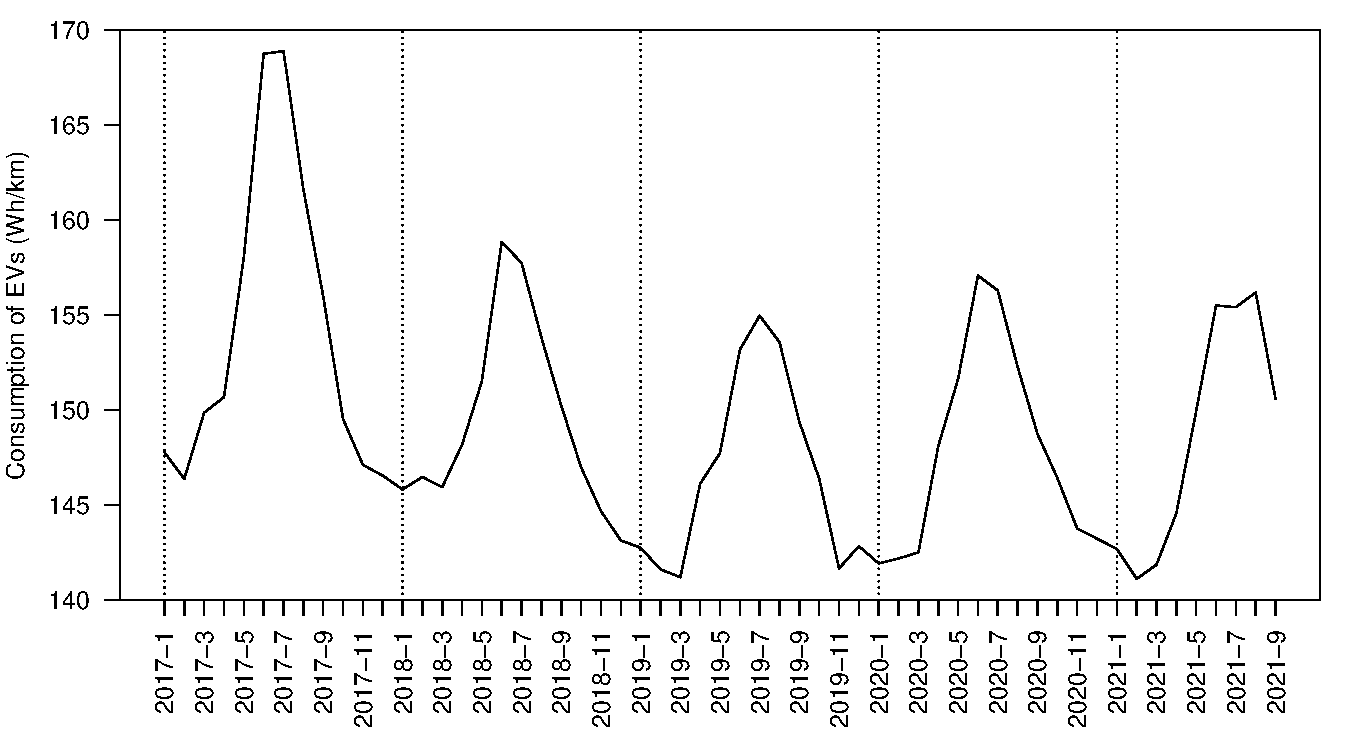
\includegraphics{final_report_Raffertys_edits_for_Vector_files/figure-latex/consum_plot-1.pdf}
\caption{National monthly average energy economy of Flip the Fleet
vehicles\label{fig:consum_plot}}
\end{figure}

Figure \ref{fig:consum_plot} shows there is a clear seasonal trend in
the national monthly average energy economy of Flip the Fleets vehicles.

A time series decomposition is used to isolate the seasonal trend in
energy economy from the overall trend. This can be done for all regions
of NZ combined and also for each region individually.

\begin{figure}
\centering
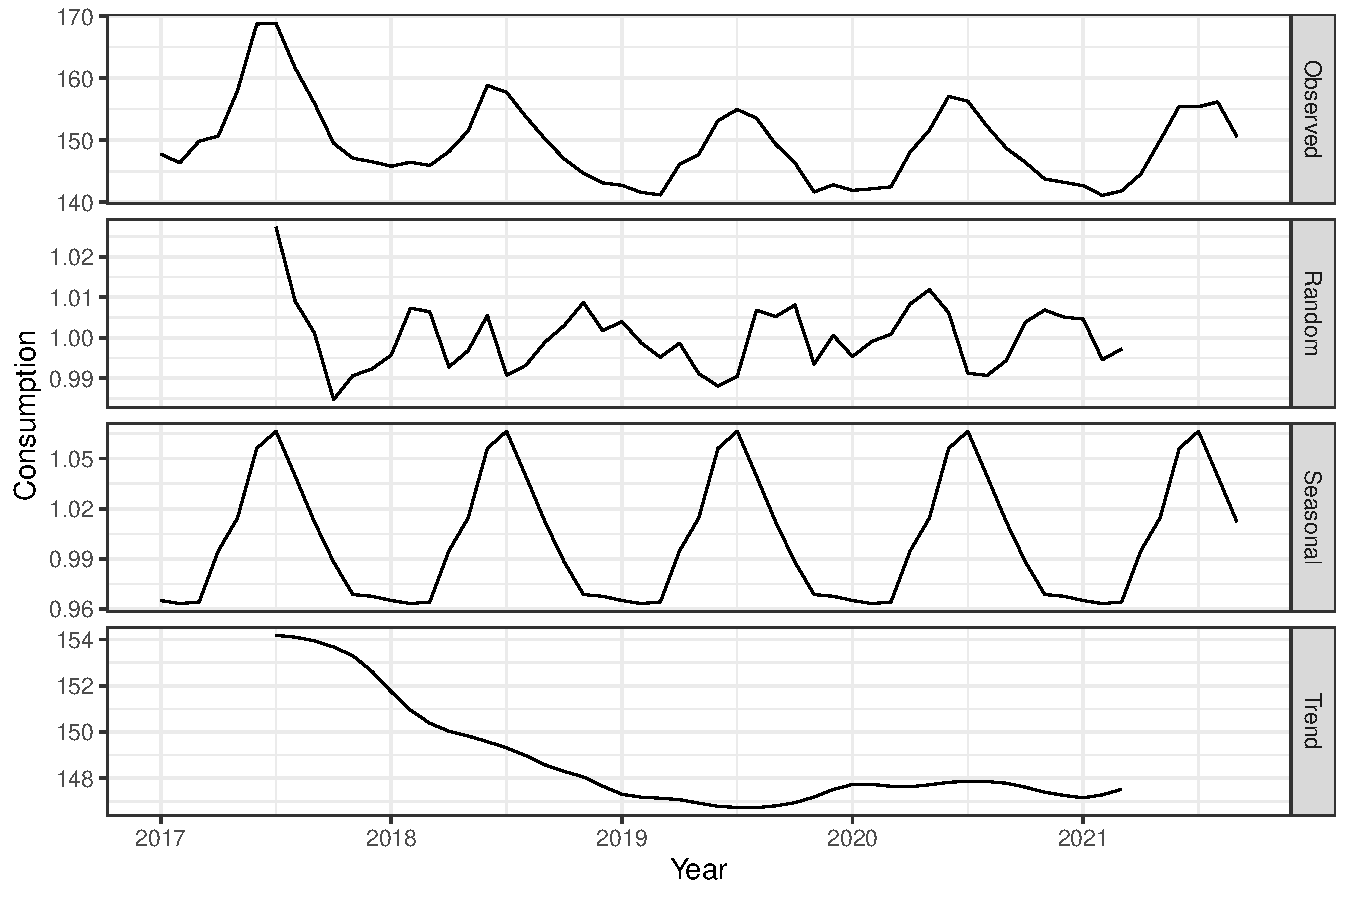
\includegraphics{final_report_Raffertys_edits_for_Vector_files/figure-latex/consum_decomp_plot-1.pdf}
\caption{Multiplicative time series decomposition of Flip the Fleet
average energy economy for all of NZ\label{fig:consum_decomp_plot}}
\end{figure}

\begin{figure}
\centering
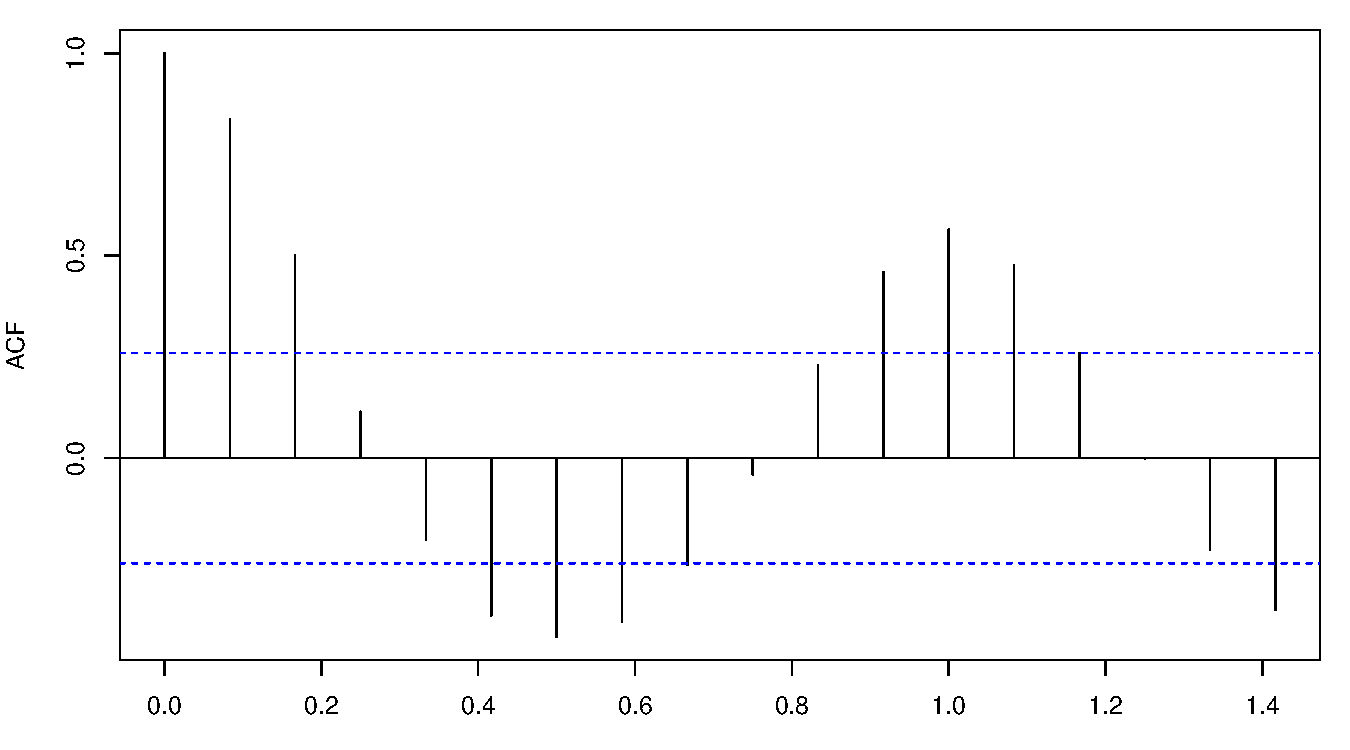
\includegraphics{final_report_Raffertys_edits_for_Vector_files/figure-latex/acf_consum-1.pdf}
\caption{Autocorrelation plot of Flip the Fleet average energy economy
for all of NZ\label{fig:acf_consum}}
\end{figure}

The time series decomposition (Figure \ref{fig:consum_decomp_plot})
shows a very clear seasonal trend. The autocorrelation plot (Figure
\ref{fig:acf_consum}) shows that this yearly trend is significant. This
seasonal trend goes from 0.96 times the mean energy economy in February
to 1.07 times the mean energy economy in July, a peak to peak difference
of 10.7\%.

\hypertarget{weather-correlations}{%
\subsubsection{Weather correlations}\label{weather-correlations}}

Past research shows that a majority of the seasonal variation in EV
efficiency is due to cabin temperature control\cite{ev_range}. This
would suggest that EV energy economy is correlated with heating degree
days. To test this hypothesis, as NZ weather differs significantly by
region, we must limit the comparison to a single region and compare it
to that regions weather at the same period of time.

In order to do this, hourly weather data from 2017 to 2021 was collected
from the NIWA National Climate Database for 14 regions around New
Zealand that best correspond to the regions of the Flip the Fleet
vehicles. Using the regional hourly temperatures, monthly heating degree
days (HDD) and cooling degree days (CDD) were imputed using base
temperatures of 16\(^\circ\)C and 22\(^\circ\)C respectively. These base
temperatures were selected to represent the range of comfortable
temperatures for most people. Monthly average temperature were also
calculated.

The HDD and CDD was then divided by the length of the month to determine
to average heating/cooling degrees days per day for the month. This is
so that there is less bias when comparing to other statistics such as
efficiency that are averaged out rather than summed.

The calculated monthly weather statistics by region was then compared to
the monthly EV data based on the regions of vehicle. This assumes that
most vehicles stay in their own region for a majority of the time.

\begin{figure}
\centering
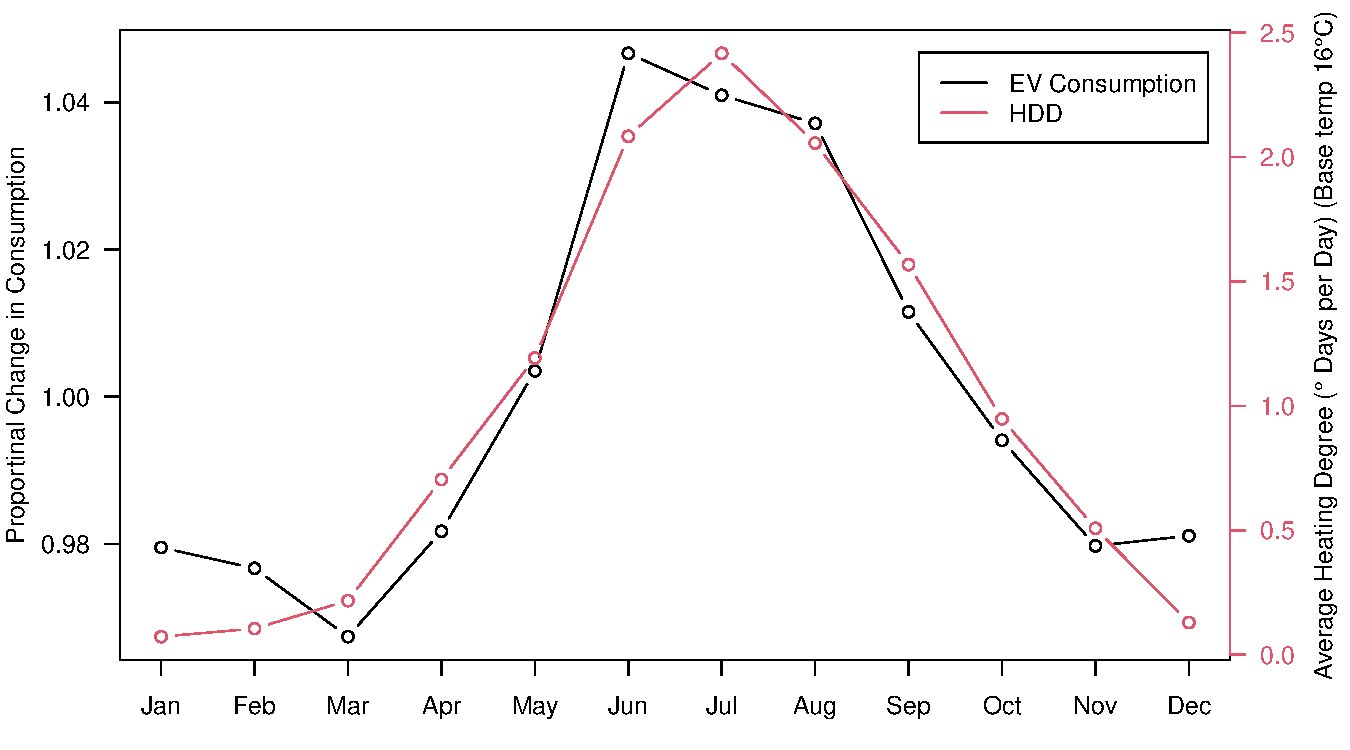
\includegraphics{final_report_Raffertys_edits_for_Vector_files/figure-latex/consum_HDD_plot-1.pdf}
\caption{Auckland seasonal HDD and EV energy economy
decompostions\label{fig:consum_HDD_plot}}
\end{figure}

Auckland is used as an example to compare correlation between HDD and
energy economy as it has the largest amount of data and is of most
interest to Vector. Within Auckland, Figure \ref{fig:consum_HDD_plot}
shows very clearly that HDD and energy economy of EVs are highly
correlated. There is a slight increase in energy economy in January and
February and it can be questioned if that is due to AC usage which would
decrease range \cite{ev_range} or other factors such as holiday travel,
often involving highway driving which EVs are generally less efficient
at \cite{ev_highway}. This effect is not obvious in the overall trend
for NZ, so is most likely due to the fact that Auckland has a warmer
climate than the rest of NZ.

\begin{figure}
\centering
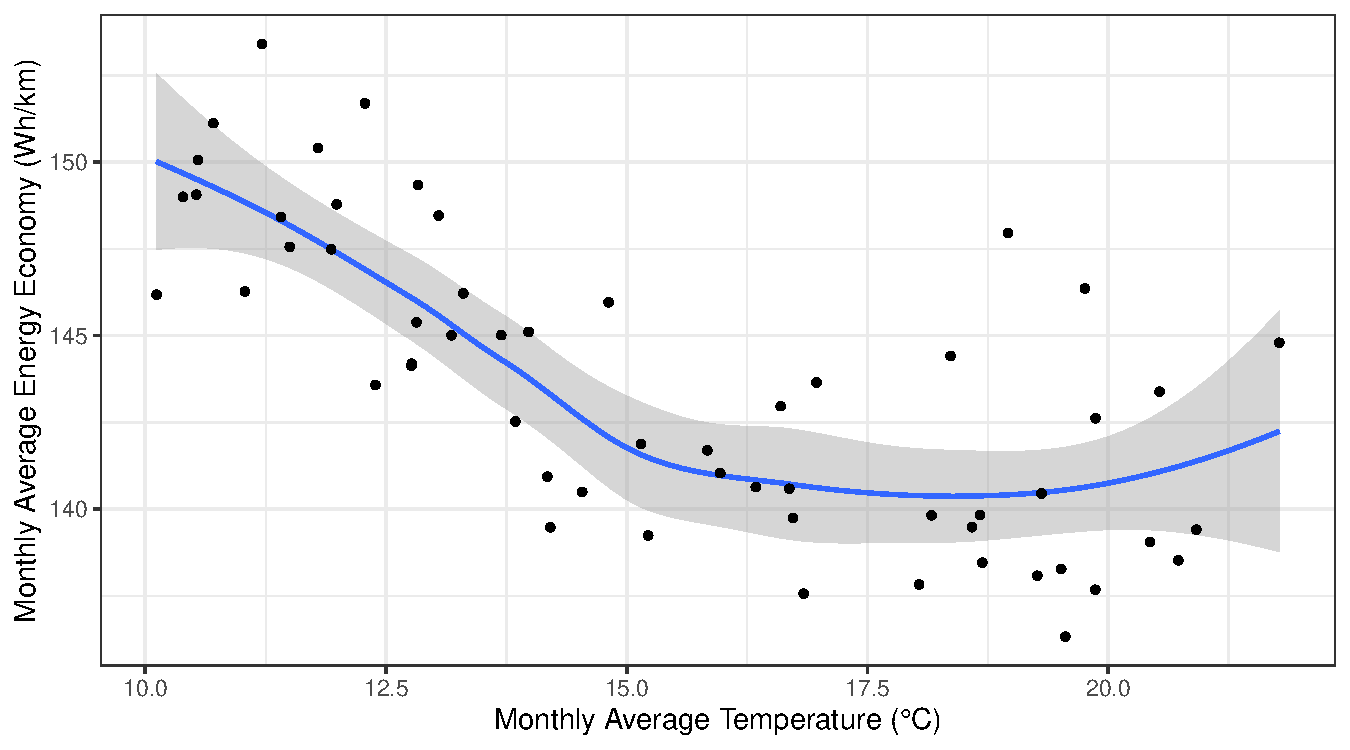
\includegraphics{final_report_Raffertys_edits_for_Vector_files/figure-latex/temp_consum_plot-1.pdf}
\caption{Auckland monthly average energy economy by avg
temperature\label{fig:temp_consum_plot}}
\end{figure}

Further exploring the relation between energy economy and weather in
Auckland, Figure \ref{fig:temp_consum_plot} shows a decreasing energy
economy up to around a monthly average temperature of 17.5°C. However,
increasing monthly average temperature past this, there appears to be a
trend towards increasing EV energy economy. As stated previously,
existing research suggests AC also increases energy economy of EVs
\cite{ev_range}. This suggests it may be worth including both cooling
degree days and heating degree days in the analysis. This could also be
useful to explain the points well above the trend line that may be from
a month where there was both cold and warm days contributing to a high
usage of cabin temperature control, increasing energy economy, but
average temperature would not be able to show this.

\hypertarget{nz-vehicle-kilometers-travelled}{%
\subsubsection{NZ vehicle kilometers
travelled}\label{nz-vehicle-kilometers-travelled}}

To determine the seasonal impacts of EV charging on our electricity
network under scenarios of increasing transport electrification we need
to understand seasonality in current driving patterns. A number of data
sets were considered including fuel usage and vehicle kilometers
traveled (VKT) data.

To explore the seasonal trend in fuel usage in NZ, fuel trade data from
the Ministry of Business, Innovation and Employment (MBIE) is used
\cite{fuel_trade}. This data set includes quarterly fuel usage data
broken down by fuel type and sector. This allows the isolation of petrol
usage in domestic land transport, which should provide an estimate of
the fuel usage by light passenger vehicles. Fuel trade data from 2020
was excluded as lockdowns were not an accurate representation of the
general driving patterns of the NZ population.

\begin{figure}
\centering
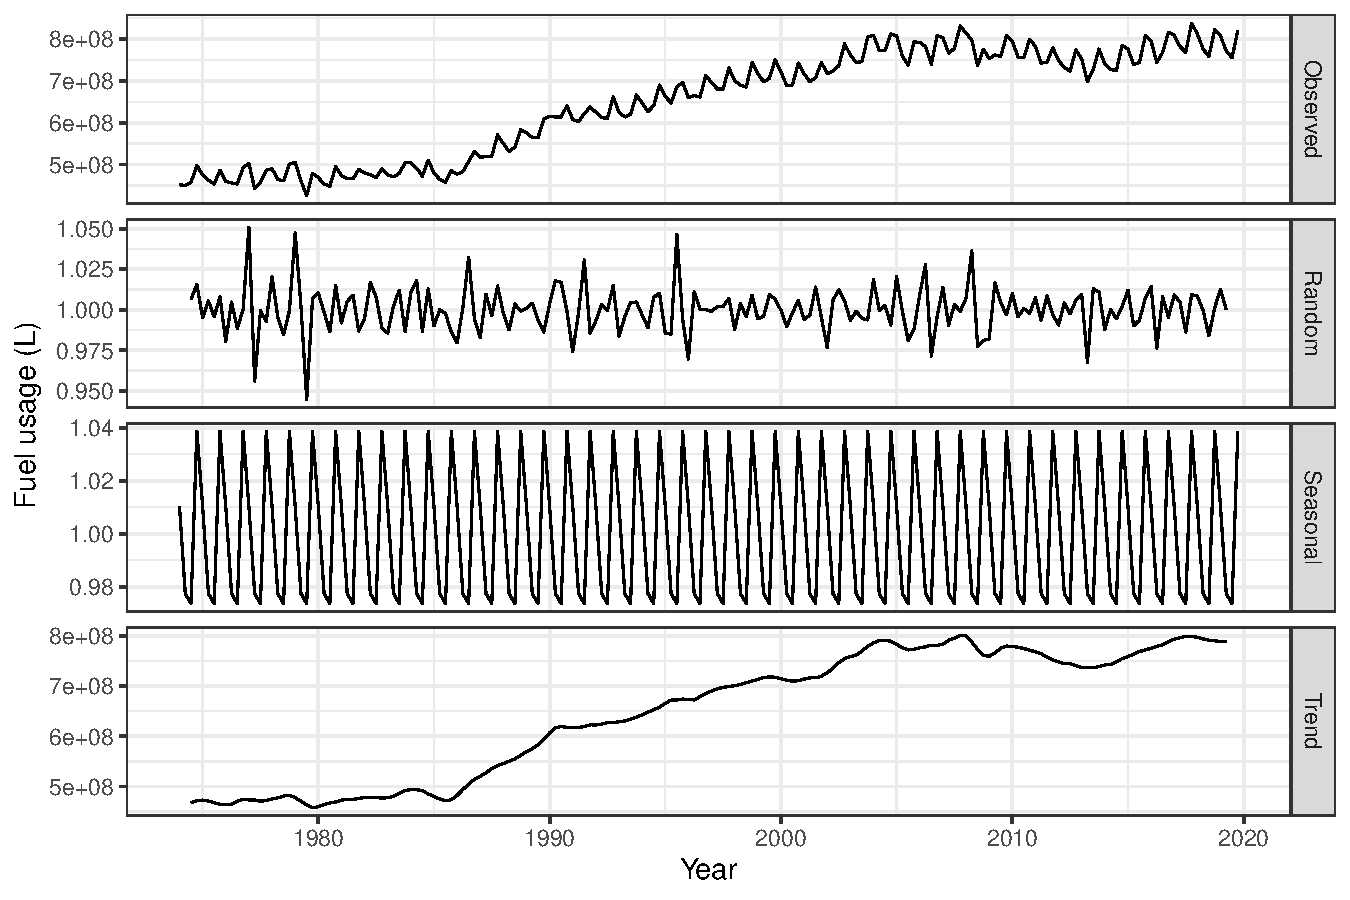
\includegraphics{final_report_Raffertys_edits_for_Vector_files/figure-latex/petrol_ts-1.pdf}
\caption{Multiplicative time series decomposition of petrol usage in
domestic land transport in NZ\label{fig:petrol_ts}}
\end{figure}

The time series decomposition in Figure \ref{fig:petrol_ts} shows a
seasonal trend in petrol usage, however it is of relatively small
magnitude compared to the random variations suggesting this trend may
not be significant.

\begin{figure}
\centering
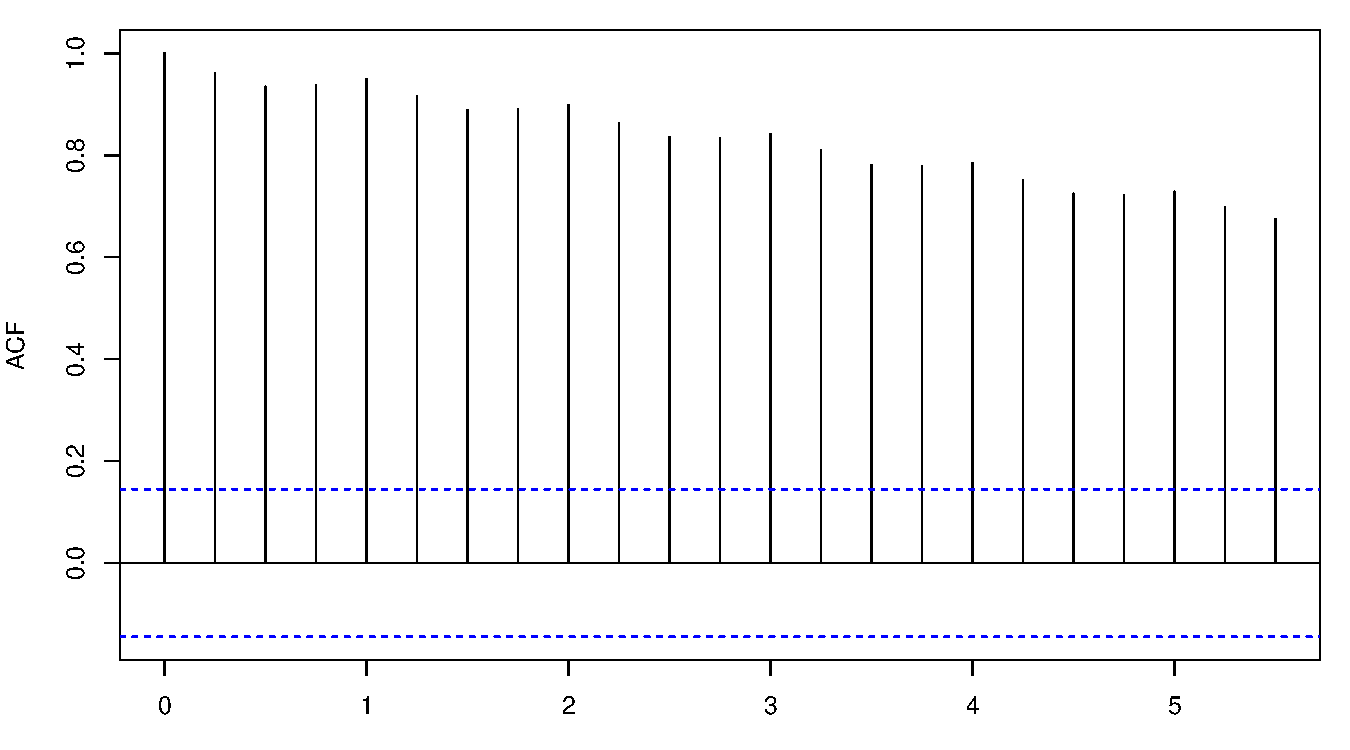
\includegraphics{final_report_Raffertys_edits_for_Vector_files/figure-latex/acf_petrol-1.pdf}
\caption{Autocorrelation of petrol usage in domestic land transport in
NZ\label{fig:acf_petrol}}
\end{figure}

The autocorrelation plot (figure \ref{fig:acf_petrol}) suggest that
there is some slight seasonality in petrol usage, however it does not
appear to be significant.

Fuel trade data can be compared to the VKT data from the Ministry of
Transport. VKT data including quarterly data of 10 regions plus one
``other'' region was given by Haobo Wang from the Ministry of Transport
for use in this project. Further yearly data for VKT of the ``other''
regions, the vehicle fuel type and vehicle type was collected from the
publicly available fleet statistics page on Ministry of Transport's
website. The quarterly VKT data was then multiplied by the proportion of
VKT that was attributed to light passenger vehicles in that year.

\begin{figure}
\centering
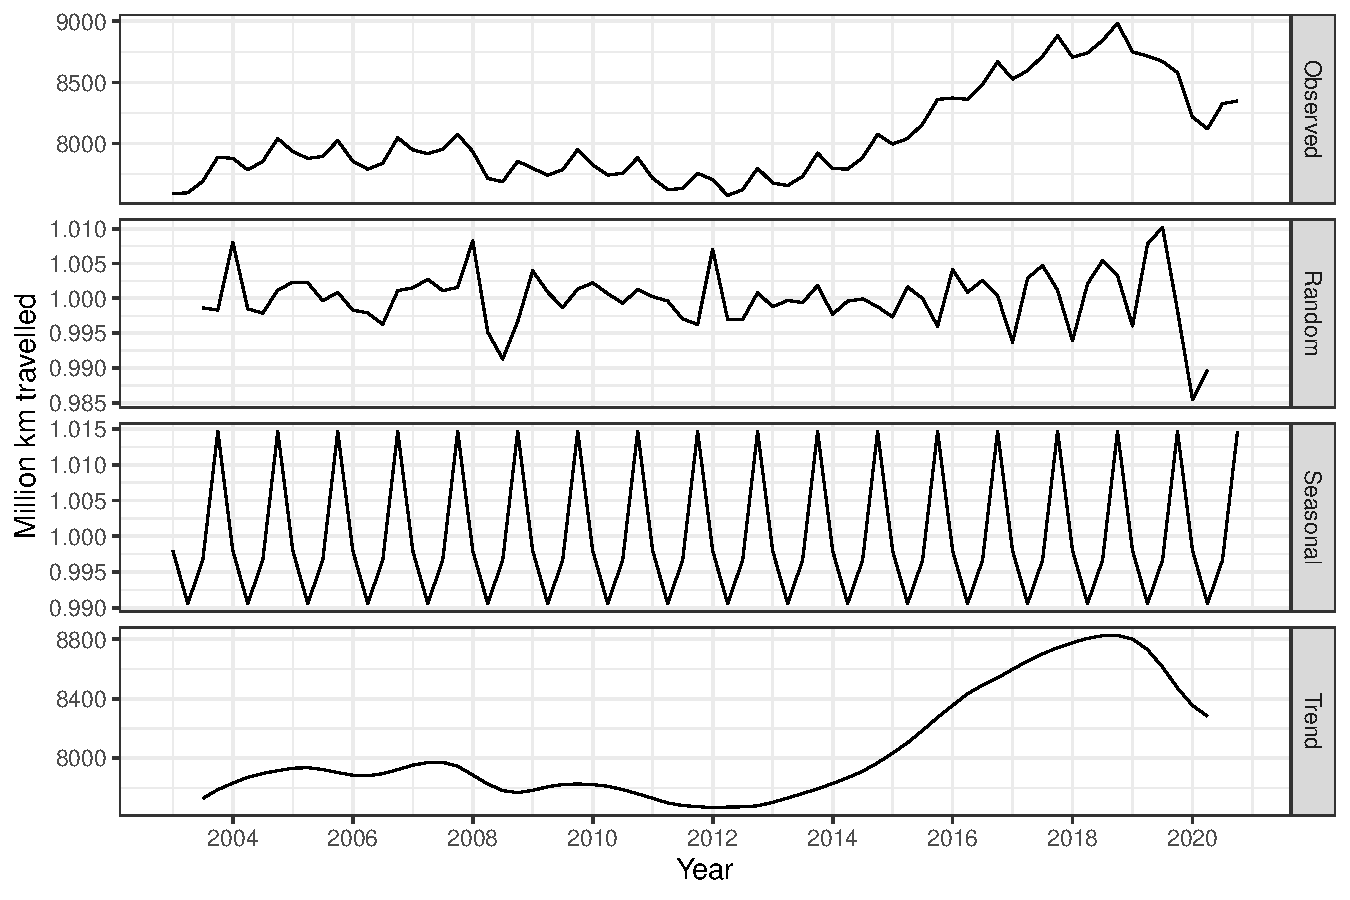
\includegraphics{final_report_Raffertys_edits_for_Vector_files/figure-latex/VKT_ts-1.pdf}
\caption{Decomposition of NZ all regions passenger VKT Time
Series\label{fig:VKT_ts}}
\end{figure}

Figure \ref{fig:VKT_ts} shows the time-series decomposition of the NZ
total VKT data, which displays a clear seasonal trend, albeit smaller
than the trend from the fuel sales data. There is, however, clearly a
large amount of smoothing going on with this data. This is shown in a
couple of different ways including:

\begin{itemize}
\item The drop of VKT due to lockdown which started in 2020 March is already visible in the data from early 2019. 
\item Related to the previous point, the random component of time series decomposition shows only a 10\% decrease in VKT spread out over a 1 year period from lockdown, compared to 30\% drop in fuel usage during only 1 quarter shown in the MIBE fuel trade data. 
\item Random variation in MIBE fuel trade data shows around a 3 times greater random variation. There could be a seasonal effect on fuel efficiency which could change the seasonal fuel trend relative to VKT, but there is no reason there would be any significant randomness in fuel efficiency so randomness should be of similar magnitude.
\end{itemize}

This smoothing likely occurs due to the method of VKT data collection
using the odometer readings during WoF/CoF. For a majority of vehicles
WoF is only done once a year and in the case of new cars that could be
up to 3 years. This likely causes the data to show less seasonal trend
than may exist in the real world.

Looking at the long term trend, VKT remained largely flat between 2004
and 2012 after which there was a steady but significant increase until
2019. After this, there is a decrease in VKT due to lockdown, which in
this data set for the above reasons likely started showing its effects
in 2019.

\begin{figure}
\centering
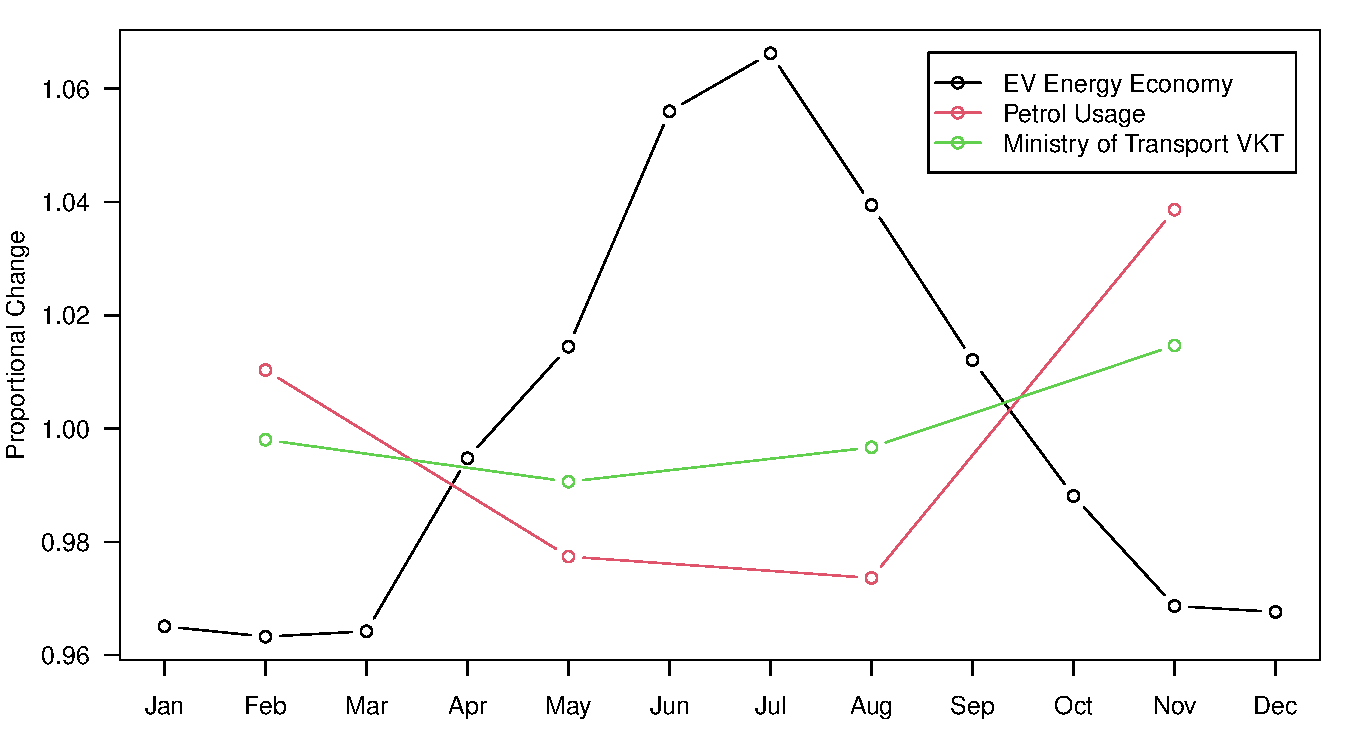
\includegraphics{final_report_Raffertys_edits_for_Vector_files/figure-latex/petrol_VKT_vs_eff-1.pdf}
\caption{NZ Seasonal Component Decompostions}
\end{figure}

Looking at the seasonal trend of petrol usage and VKT data from The
Ministry of Transport, we can see an obvious decrease in the winter
months with a peak in the 4th quarter likely corresponding to holiday
travel. Petrol usage shows this variation to be much larger in the VKT
data from Ministry of Transport. It is unclear whether this would be due
to the smoothing effect as was previously discussed regarding the
Ministry of Transport data, or perhaps a change in efficiency for petrol
vehicle by seasons similar to that of the EV. Combining these 2 data
sets it is reasonable to suggest that in New Zealand, compared to the
winter (Q2 and Q3) VKT, the true VKT in the summer (Q1 and Q4) is
between 1.3\% higher, as suggested by the VKT data from Ministry of
Transport, to 5\% higher, according to the petrol usage data.

Looking at the seasonal trend of EV energy economy we can see a much
larger increase in energy economy in the winter months, with average
energy economy in July being 10.7\% higher than in February. From the
plot we can see that when energy economy of EVs increases, VKT goes
down, suggesting that some increase in total power usage due to EVs
increase in energy economy will be countered by a decrease in VKT.
However, the increase in energy economy is much larger than the decrease
in VKT. This, combined with the fact that winter is when our electricity
grid in New Zealand is already under strain due to heating demand,
suggests that if we ignore the relatively small change in VKT in our
model we can effectively model a worst case scenario. Thus we propose
that monthly distance (\(d_{R}\)) in our model is constant and
determined by the yearly regional VKT data from 2019.

\hypertarget{model}{%
\subsection{Model}\label{model}}

Based on the findings from the data exploration, we propose EV
electricity demand (\(E_{m,R}\)) for each month and region is given by
the formula:

\begin{equation}
\label{eq:energy_usage}
E_{m,R} = \sum_{C} F_C \times \eta_{m,R,C} \times d_{R}
\end{equation}

Where \(F_C\) is the proportion of model in the fleet, and
\(\eta_{m,R,C}\) is the monthly region energy economy of a particular
vehicle model. As stated in the data exploration section monthly
distance (\(d_{R}\)) in our model is determined from the yearly regional
VKT data from 2019 and has no monthly dependency.

Based on the data exploration we propose we model EV energy economy
(\(\eta_{m,R,C}\)) using a linear model given by the formula:

\begin{equation}
\label{eq:linear_model}
\eta_{m,R,C} = \beta_{CDD}{CDD}_{m,R} + \beta_{HDD}{HDD}_{m,R} + K_R + L_C + \beta_0 + \epsilon
\end{equation}

where \({CDD}_{m,R}\) and \({HDD}_{m,R}\) is the number of CDD and HDD
each month in each region, \(K_R\) is a constant given for each region,
\(L_C\) is a constant given for each model of car and \(\beta_0\) is a
constant intercept. This means \emph{expected} energy economy can be
given by the formula:

\begin{equation}
\label{eq:economy_model}
\eta_{m,R,C} = \beta_{CDD}{CDD}_{m,R} + \beta_{HDD}{HDD}_{m,R} + B_{R,C}
\end{equation}

where \(B_{R,C} = K_R + L_C + \beta_0\) and is effectively a baseline
efficiency of a particular vehicle model in a particular region with no
HDD or CDD related impacts.

A different intercept is used for each model of car as a majority of the
variation in efficiency will be due to different vehicle models.
Including the vehicle model therefore allows for much better model fit
and smaller confidence intervals. A different intercept is also used for
each weather region as weather might be measured in a cold or hot
section of region. Also, the region may have more or less hill/highway
which could influence driving patterns impacting efficiency. However the
gradients of the HDD term (\(\beta_{HDD}\)) and CDD
term(\(\beta_{CDD}\)) are kept the same for all regions and models as
this is the number that determines how HDD and CDD affect the efficiency
of the EV.

As with the case of the adjusted monthly average power energy economy
(Wh/km) in the linear model, a weighting is added to the points in order
to give more weighting to cars with longer distance traveled.
Mathematically, this means that instead of estimating the coefficients
by minimizing the residual sum of squares (RSS) given by the function
\(\sum_{i =1}^{n}(\eta_{i}-\hat{\eta}_{i})^2\), we instead minimize the
function \(\sum_{i =1}^{n}d \cdot(\eta_{i}-\hat{\eta}_{i})^2\), where
\(d\) is the distance traveled by a car in that month, \(\eta_{i}\) is
the actual power energy economy, and \(\hat{\eta}_{i}\) is the power
energy economy of that vehicle as predicted by the model.

EV energy economy is modelled with a linear model as with the correct
base temperature, the usage of power to warm/cool the cabin should be
roughly linear to the HDD/CDD \cite{HDD_est}. This would allow energy
used to heat/cool the car to be isolated for analysis from drivetrain
power energy economy. Conceptually it makes sense that extra power usage
due to heating/cooling demand to be independent from drivetrain demand
as unlike in traditional internal combustion engine (ICE) vehicles where
the energy to heat and cool the cabin comes from the engine, an EVs heat
pump or resistive heater and AC can draw power from the battery
independently of the engine. Unfortunately, this linear correlation may
break down as cars unlike houses or buildings are often only used at
particular hours of the day for short periods. This means the
correlation may have more dependency towards the temperature at times
such as the morning or evening commute hours, the modelling of which
would require higher resolution data than we have available.

\begin{longtable}[]{@{}lrrrr@{}}
\toprule
\begin{minipage}[b]{0.35\columnwidth}\raggedright
~\strut
\end{minipage} & \begin{minipage}[b]{0.12\columnwidth}\raggedleft
Estimate\strut
\end{minipage} & \begin{minipage}[b]{0.14\columnwidth}\raggedleft
Std. Error\strut
\end{minipage} & \begin{minipage}[b]{0.11\columnwidth}\raggedleft
t value\strut
\end{minipage} & \begin{minipage}[b]{0.14\columnwidth}\raggedleft
Pr(\textgreater\textbar t\textbar)\strut
\end{minipage}\tabularnewline
\midrule
\endhead
\begin{minipage}[t]{0.35\columnwidth}\raggedright
(Intercept)\strut
\end{minipage} & \begin{minipage}[t]{0.12\columnwidth}\raggedleft
132.1\strut
\end{minipage} & \begin{minipage}[t]{0.14\columnwidth}\raggedleft
0.2867\strut
\end{minipage} & \begin{minipage}[t]{0.11\columnwidth}\raggedleft
460.8\strut
\end{minipage} & \begin{minipage}[t]{0.14\columnwidth}\raggedleft
0\strut
\end{minipage}\tabularnewline
\begin{minipage}[t]{0.35\columnwidth}\raggedright
HDD\strut
\end{minipage} & \begin{minipage}[t]{0.12\columnwidth}\raggedleft
2.195\strut
\end{minipage} & \begin{minipage}[t]{0.14\columnwidth}\raggedleft
0.05096\strut
\end{minipage} & \begin{minipage}[t]{0.11\columnwidth}\raggedleft
43.07\strut
\end{minipage} & \begin{minipage}[t]{0.14\columnwidth}\raggedleft
0\strut
\end{minipage}\tabularnewline
\begin{minipage}[t]{0.35\columnwidth}\raggedright
CDD\strut
\end{minipage} & \begin{minipage}[t]{0.12\columnwidth}\raggedleft
2.347\strut
\end{minipage} & \begin{minipage}[t]{0.14\columnwidth}\raggedleft
0.5722\strut
\end{minipage} & \begin{minipage}[t]{0.11\columnwidth}\raggedleft
4.102\strut
\end{minipage} & \begin{minipage}[t]{0.14\columnwidth}\raggedleft
4.113e-05\strut
\end{minipage}\tabularnewline
\begin{minipage}[t]{0.35\columnwidth}\raggedright
Region\_Upper Hutt\strut
\end{minipage} & \begin{minipage}[t]{0.12\columnwidth}\raggedleft
-0.4796\strut
\end{minipage} & \begin{minipage}[t]{0.14\columnwidth}\raggedleft
0.3036\strut
\end{minipage} & \begin{minipage}[t]{0.11\columnwidth}\raggedleft
-1.58\strut
\end{minipage} & \begin{minipage}[t]{0.14\columnwidth}\raggedleft
0.1141\strut
\end{minipage}\tabularnewline
\begin{minipage}[t]{0.35\columnwidth}\raggedright
Region\_Christchurch\strut
\end{minipage} & \begin{minipage}[t]{0.12\columnwidth}\raggedleft
-0.9073\strut
\end{minipage} & \begin{minipage}[t]{0.14\columnwidth}\raggedleft
0.3257\strut
\end{minipage} & \begin{minipage}[t]{0.11\columnwidth}\raggedleft
-2.786\strut
\end{minipage} & \begin{minipage}[t]{0.14\columnwidth}\raggedleft
0.005348\strut
\end{minipage}\tabularnewline
\begin{minipage}[t]{0.35\columnwidth}\raggedright
Region\_Dunedin\strut
\end{minipage} & \begin{minipage}[t]{0.12\columnwidth}\raggedleft
12.06\strut
\end{minipage} & \begin{minipage}[t]{0.14\columnwidth}\raggedleft
0.3835\strut
\end{minipage} & \begin{minipage}[t]{0.11\columnwidth}\raggedleft
31.45\strut
\end{minipage} & \begin{minipage}[t]{0.14\columnwidth}\raggedleft
1.705e-212\strut
\end{minipage}\tabularnewline
\begin{minipage}[t]{0.35\columnwidth}\raggedright
Region\_Hamilton\strut
\end{minipage} & \begin{minipage}[t]{0.12\columnwidth}\raggedleft
8.513\strut
\end{minipage} & \begin{minipage}[t]{0.14\columnwidth}\raggedleft
0.5298\strut
\end{minipage} & \begin{minipage}[t]{0.11\columnwidth}\raggedleft
16.07\strut
\end{minipage} & \begin{minipage}[t]{0.14\columnwidth}\raggedleft
8.999e-58\strut
\end{minipage}\tabularnewline
\begin{minipage}[t]{0.35\columnwidth}\raggedright
Region\_Nelson\strut
\end{minipage} & \begin{minipage}[t]{0.12\columnwidth}\raggedleft
2.711\strut
\end{minipage} & \begin{minipage}[t]{0.14\columnwidth}\raggedleft
0.4806\strut
\end{minipage} & \begin{minipage}[t]{0.11\columnwidth}\raggedleft
5.642\strut
\end{minipage} & \begin{minipage}[t]{0.14\columnwidth}\raggedleft
1.7e-08\strut
\end{minipage}\tabularnewline
\begin{minipage}[t]{0.35\columnwidth}\raggedright
Region\_Rotorua\strut
\end{minipage} & \begin{minipage}[t]{0.12\columnwidth}\raggedleft
5.015\strut
\end{minipage} & \begin{minipage}[t]{0.14\columnwidth}\raggedleft
0.5462\strut
\end{minipage} & \begin{minipage}[t]{0.11\columnwidth}\raggedleft
9.182\strut
\end{minipage} & \begin{minipage}[t]{0.14\columnwidth}\raggedleft
4.597e-20\strut
\end{minipage}\tabularnewline
\begin{minipage}[t]{0.35\columnwidth}\raggedright
Region\_Clyde\strut
\end{minipage} & \begin{minipage}[t]{0.12\columnwidth}\raggedleft
4.53\strut
\end{minipage} & \begin{minipage}[t]{0.14\columnwidth}\raggedleft
0.7491\strut
\end{minipage} & \begin{minipage}[t]{0.11\columnwidth}\raggedleft
6.048\strut
\end{minipage} & \begin{minipage}[t]{0.14\columnwidth}\raggedleft
1.494e-09\strut
\end{minipage}\tabularnewline
\begin{minipage}[t]{0.35\columnwidth}\raggedright
Region\_Palmerston North\strut
\end{minipage} & \begin{minipage}[t]{0.12\columnwidth}\raggedleft
14.11\strut
\end{minipage} & \begin{minipage}[t]{0.14\columnwidth}\raggedleft
0.6652\strut
\end{minipage} & \begin{minipage}[t]{0.11\columnwidth}\raggedleft
21.21\strut
\end{minipage} & \begin{minipage}[t]{0.14\columnwidth}\raggedleft
6.519e-99\strut
\end{minipage}\tabularnewline
\begin{minipage}[t]{0.35\columnwidth}\raggedright
Region\_Stratford\strut
\end{minipage} & \begin{minipage}[t]{0.12\columnwidth}\raggedleft
10.36\strut
\end{minipage} & \begin{minipage}[t]{0.14\columnwidth}\raggedleft
0.9497\strut
\end{minipage} & \begin{minipage}[t]{0.11\columnwidth}\raggedleft
10.91\strut
\end{minipage} & \begin{minipage}[t]{0.14\columnwidth}\raggedleft
1.254e-27\strut
\end{minipage}\tabularnewline
\begin{minipage}[t]{0.35\columnwidth}\raggedright
Region\_Napier\strut
\end{minipage} & \begin{minipage}[t]{0.12\columnwidth}\raggedleft
6.316\strut
\end{minipage} & \begin{minipage}[t]{0.14\columnwidth}\raggedleft
0.8473\strut
\end{minipage} & \begin{minipage}[t]{0.11\columnwidth}\raggedleft
7.455\strut
\end{minipage} & \begin{minipage}[t]{0.14\columnwidth}\raggedleft
9.311e-14\strut
\end{minipage}\tabularnewline
\begin{minipage}[t]{0.35\columnwidth}\raggedright
Region\_Invercargill\strut
\end{minipage} & \begin{minipage}[t]{0.12\columnwidth}\raggedleft
3.191\strut
\end{minipage} & \begin{minipage}[t]{0.14\columnwidth}\raggedleft
1.758\strut
\end{minipage} & \begin{minipage}[t]{0.11\columnwidth}\raggedleft
1.815\strut
\end{minipage} & \begin{minipage}[t]{0.14\columnwidth}\raggedleft
0.06949\strut
\end{minipage}\tabularnewline
\begin{minipage}[t]{0.35\columnwidth}\raggedright
Model\_Nissan Leaf (30 kWh)\strut
\end{minipage} & \begin{minipage}[t]{0.12\columnwidth}\raggedleft
3.401\strut
\end{minipage} & \begin{minipage}[t]{0.14\columnwidth}\raggedleft
0.2524\strut
\end{minipage} & \begin{minipage}[t]{0.11\columnwidth}\raggedleft
13.47\strut
\end{minipage} & \begin{minipage}[t]{0.14\columnwidth}\raggedleft
3.276e-41\strut
\end{minipage}\tabularnewline
\begin{minipage}[t]{0.35\columnwidth}\raggedright
Model\_Nissan Leaf (24 kWh) 2011-2012\strut
\end{minipage} & \begin{minipage}[t]{0.12\columnwidth}\raggedleft
12.39\strut
\end{minipage} & \begin{minipage}[t]{0.14\columnwidth}\raggedleft
0.3246\strut
\end{minipage} & \begin{minipage}[t]{0.11\columnwidth}\raggedleft
38.17\strut
\end{minipage} & \begin{minipage}[t]{0.14\columnwidth}\raggedleft
7.229e-309\strut
\end{minipage}\tabularnewline
\begin{minipage}[t]{0.35\columnwidth}\raggedright
Model\_Nissan Leaf (40 kWh)\strut
\end{minipage} & \begin{minipage}[t]{0.12\columnwidth}\raggedleft
10.68\strut
\end{minipage} & \begin{minipage}[t]{0.14\columnwidth}\raggedleft
0.5174\strut
\end{minipage} & \begin{minipage}[t]{0.11\columnwidth}\raggedleft
20.63\strut
\end{minipage} & \begin{minipage}[t]{0.14\columnwidth}\raggedleft
1.046e-93\strut
\end{minipage}\tabularnewline
\begin{minipage}[t]{0.35\columnwidth}\raggedright
Model\_Nissan e-NV200 (24 kWh)\strut
\end{minipage} & \begin{minipage}[t]{0.12\columnwidth}\raggedleft
32.71\strut
\end{minipage} & \begin{minipage}[t]{0.14\columnwidth}\raggedleft
0.5367\strut
\end{minipage} & \begin{minipage}[t]{0.11\columnwidth}\raggedleft
60.95\strut
\end{minipage} & \begin{minipage}[t]{0.14\columnwidth}\raggedleft
0\strut
\end{minipage}\tabularnewline
\begin{minipage}[t]{0.35\columnwidth}\raggedright
Model\_Hyundai Ioniq (EV)\strut
\end{minipage} & \begin{minipage}[t]{0.12\columnwidth}\raggedleft
-18.32\strut
\end{minipage} & \begin{minipage}[t]{0.14\columnwidth}\raggedleft
0.685\strut
\end{minipage} & \begin{minipage}[t]{0.11\columnwidth}\raggedleft
-26.75\strut
\end{minipage} & \begin{minipage}[t]{0.14\columnwidth}\raggedleft
3.342e-155\strut
\end{minipage}\tabularnewline
\begin{minipage}[t]{0.35\columnwidth}\raggedright
Model\_BMW i3\strut
\end{minipage} & \begin{minipage}[t]{0.12\columnwidth}\raggedleft
-1.335\strut
\end{minipage} & \begin{minipage}[t]{0.14\columnwidth}\raggedleft
0.7873\strut
\end{minipage} & \begin{minipage}[t]{0.11\columnwidth}\raggedleft
-1.695\strut
\end{minipage} & \begin{minipage}[t]{0.14\columnwidth}\raggedleft
0.09006\strut
\end{minipage}\tabularnewline
\begin{minipage}[t]{0.35\columnwidth}\raggedright
Model\_Hyundai Kona (EV)\strut
\end{minipage} & \begin{minipage}[t]{0.12\columnwidth}\raggedleft
0.6822\strut
\end{minipage} & \begin{minipage}[t]{0.14\columnwidth}\raggedleft
0.86\strut
\end{minipage} & \begin{minipage}[t]{0.11\columnwidth}\raggedleft
0.7933\strut
\end{minipage} & \begin{minipage}[t]{0.14\columnwidth}\raggedleft
0.4276\strut
\end{minipage}\tabularnewline
\begin{minipage}[t]{0.35\columnwidth}\raggedright
Model\_Renault Zoe\strut
\end{minipage} & \begin{minipage}[t]{0.12\columnwidth}\raggedleft
11.55\strut
\end{minipage} & \begin{minipage}[t]{0.14\columnwidth}\raggedleft
0.8507\strut
\end{minipage} & \begin{minipage}[t]{0.11\columnwidth}\raggedleft
13.57\strut
\end{minipage} & \begin{minipage}[t]{0.14\columnwidth}\raggedleft
8.383e-42\strut
\end{minipage}\tabularnewline
\begin{minipage}[t]{0.35\columnwidth}\raggedright
Model\_Tesla Model 3\strut
\end{minipage} & \begin{minipage}[t]{0.12\columnwidth}\raggedleft
10.55\strut
\end{minipage} & \begin{minipage}[t]{0.14\columnwidth}\raggedleft
1.022\strut
\end{minipage} & \begin{minipage}[t]{0.11\columnwidth}\raggedleft
10.32\strut
\end{minipage} & \begin{minipage}[t]{0.14\columnwidth}\raggedleft
6.485e-25\strut
\end{minipage}\tabularnewline
\begin{minipage}[t]{0.35\columnwidth}\raggedright
Model\_Nissan Leaf (62 kWh)\strut
\end{minipage} & \begin{minipage}[t]{0.12\columnwidth}\raggedleft
25.46\strut
\end{minipage} & \begin{minipage}[t]{0.14\columnwidth}\raggedleft
1.752\strut
\end{minipage} & \begin{minipage}[t]{0.11\columnwidth}\raggedleft
14.53\strut
\end{minipage} & \begin{minipage}[t]{0.14\columnwidth}\raggedleft
1.295e-47\strut
\end{minipage}\tabularnewline
\begin{minipage}[t]{0.35\columnwidth}\raggedright
Model\_Kia Niro (EV)\strut
\end{minipage} & \begin{minipage}[t]{0.12\columnwidth}\raggedleft
11.34\strut
\end{minipage} & \begin{minipage}[t]{0.14\columnwidth}\raggedleft
1.193\strut
\end{minipage} & \begin{minipage}[t]{0.11\columnwidth}\raggedleft
9.511\strut
\end{minipage} & \begin{minipage}[t]{0.14\columnwidth}\raggedleft
2.075e-21\strut
\end{minipage}\tabularnewline
\begin{minipage}[t]{0.35\columnwidth}\raggedright
Model\_Tesla Model S\strut
\end{minipage} & \begin{minipage}[t]{0.12\columnwidth}\raggedleft
48.38\strut
\end{minipage} & \begin{minipage}[t]{0.14\columnwidth}\raggedleft
1.69\strut
\end{minipage} & \begin{minipage}[t]{0.11\columnwidth}\raggedleft
28.63\strut
\end{minipage} & \begin{minipage}[t]{0.14\columnwidth}\raggedleft
4.806e-177\strut
\end{minipage}\tabularnewline
\begin{minipage}[t]{0.35\columnwidth}\raggedright
Model\_Volkswagen e-Golf\strut
\end{minipage} & \begin{minipage}[t]{0.12\columnwidth}\raggedleft
1.208\strut
\end{minipage} & \begin{minipage}[t]{0.14\columnwidth}\raggedleft
1.538\strut
\end{minipage} & \begin{minipage}[t]{0.11\columnwidth}\raggedleft
0.7853\strut
\end{minipage} & \begin{minipage}[t]{0.14\columnwidth}\raggedleft
0.4323\strut
\end{minipage}\tabularnewline
\begin{minipage}[t]{0.35\columnwidth}\raggedright
Model\_Tesla Model-X\strut
\end{minipage} & \begin{minipage}[t]{0.12\columnwidth}\raggedleft
104.1\strut
\end{minipage} & \begin{minipage}[t]{0.14\columnwidth}\raggedleft
1.296\strut
\end{minipage} & \begin{minipage}[t]{0.11\columnwidth}\raggedleft
80.34\strut
\end{minipage} & \begin{minipage}[t]{0.14\columnwidth}\raggedleft
0\strut
\end{minipage}\tabularnewline
\begin{minipage}[t]{0.35\columnwidth}\raggedright
Model\_Kia Soul\strut
\end{minipage} & \begin{minipage}[t]{0.12\columnwidth}\raggedleft
6.276\strut
\end{minipage} & \begin{minipage}[t]{0.14\columnwidth}\raggedleft
1.25\strut
\end{minipage} & \begin{minipage}[t]{0.11\columnwidth}\raggedleft
5.022\strut
\end{minipage} & \begin{minipage}[t]{0.14\columnwidth}\raggedleft
5.15e-07\strut
\end{minipage}\tabularnewline
\begin{minipage}[t]{0.35\columnwidth}\raggedright
Model\_MG ZS EV\strut
\end{minipage} & \begin{minipage}[t]{0.12\columnwidth}\raggedleft
22.12\strut
\end{minipage} & \begin{minipage}[t]{0.14\columnwidth}\raggedleft
3.9\strut
\end{minipage} & \begin{minipage}[t]{0.11\columnwidth}\raggedleft
5.671\strut
\end{minipage} & \begin{minipage}[t]{0.14\columnwidth}\raggedleft
1.439e-08\strut
\end{minipage}\tabularnewline
\begin{minipage}[t]{0.35\columnwidth}\raggedright
Model\_Renault Kangoo (van)\strut
\end{minipage} & \begin{minipage}[t]{0.12\columnwidth}\raggedleft
56.63\strut
\end{minipage} & \begin{minipage}[t]{0.14\columnwidth}\raggedleft
1.537\strut
\end{minipage} & \begin{minipage}[t]{0.11\columnwidth}\raggedleft
36.84\strut
\end{minipage} & \begin{minipage}[t]{0.14\columnwidth}\raggedleft
1.301e-288\strut
\end{minipage}\tabularnewline
\begin{minipage}[t]{0.35\columnwidth}\raggedright
Model\_Jaguar I-PACE\strut
\end{minipage} & \begin{minipage}[t]{0.12\columnwidth}\raggedleft
73.02\strut
\end{minipage} & \begin{minipage}[t]{0.14\columnwidth}\raggedleft
2.951\strut
\end{minipage} & \begin{minipage}[t]{0.11\columnwidth}\raggedleft
24.75\strut
\end{minipage} & \begin{minipage}[t]{0.14\columnwidth}\raggedleft
1.949e-133\strut
\end{minipage}\tabularnewline
\begin{minipage}[t]{0.35\columnwidth}\raggedright
Model\_Peugeot e-208\strut
\end{minipage} & \begin{minipage}[t]{0.12\columnwidth}\raggedleft
10.96\strut
\end{minipage} & \begin{minipage}[t]{0.14\columnwidth}\raggedleft
9.581\strut
\end{minipage} & \begin{minipage}[t]{0.11\columnwidth}\raggedleft
1.144\strut
\end{minipage} & \begin{minipage}[t]{0.14\columnwidth}\raggedleft
0.2525\strut
\end{minipage}\tabularnewline
\bottomrule
\end{longtable}

\begin{longtable}[]{@{}rrrr@{}}
\caption{Fitting linear model: economy \textasciitilde{} HDD + CDD +
Region\_ + Model\_}\tabularnewline
\toprule
\begin{minipage}[b]{0.18\columnwidth}\raggedleft
Observations\strut
\end{minipage} & \begin{minipage}[b]{0.27\columnwidth}\raggedleft
Residual Std. Error\strut
\end{minipage} & \begin{minipage}[b]{0.11\columnwidth}\raggedleft
\(R^2\)\strut
\end{minipage} & \begin{minipage}[b]{0.21\columnwidth}\raggedleft
Adjusted \(R^2\)\strut
\end{minipage}\tabularnewline
\midrule
\endfirsthead
\toprule
\begin{minipage}[b]{0.18\columnwidth}\raggedleft
Observations\strut
\end{minipage} & \begin{minipage}[b]{0.27\columnwidth}\raggedleft
Residual Std. Error\strut
\end{minipage} & \begin{minipage}[b]{0.11\columnwidth}\raggedleft
\(R^2\)\strut
\end{minipage} & \begin{minipage}[b]{0.21\columnwidth}\raggedleft
Adjusted \(R^2\)\strut
\end{minipage}\tabularnewline
\midrule
\endhead
\begin{minipage}[t]{0.18\columnwidth}\raggedleft
22592\strut
\end{minipage} & \begin{minipage}[t]{0.27\columnwidth}\raggedleft
492.2\strut
\end{minipage} & \begin{minipage}[t]{0.11\columnwidth}\raggedleft
0.4855\strut
\end{minipage} & \begin{minipage}[t]{0.21\columnwidth}\raggedleft
0.4848\strut
\end{minipage}\tabularnewline
\bottomrule
\end{longtable}

\hypertarget{how-to-read-this-table}{%
\paragraph{How to read this table:}\label{how-to-read-this-table}}

When computing the linear model as Auckland and Nissan Leaf (24 kWh)
2013-2016 are the most common region and model they are used for the
intercept. In order to get the expected energy economy of a vehicle we
start with the (Intercept) Estimate. We then add to this energy economy
estimate the corresponding region and model Estimate (not needed if it
is Auckland or Nissan Leaf (24 kWh) 2013-2016). Number of HDD per day is
then multiplied by the HDD Estimate from the table and added to the
energy economy estimate. Similarly for CDD days number of CDD per day is
then multiplied by the CDD Estimate from the table and added to this
energy economy estimate.

The HDD term suggests that as the average number of heating degree days
per day increases by 1, the average energy economy of EVs for the month
increases by 2.19Wh/km. The CDD term suggests that as the average number
of cooling degree days per days increases by 1 the average power energy
economy of EVs for the month increases by 2.35Wh/km.

\begin{figure}
\centering
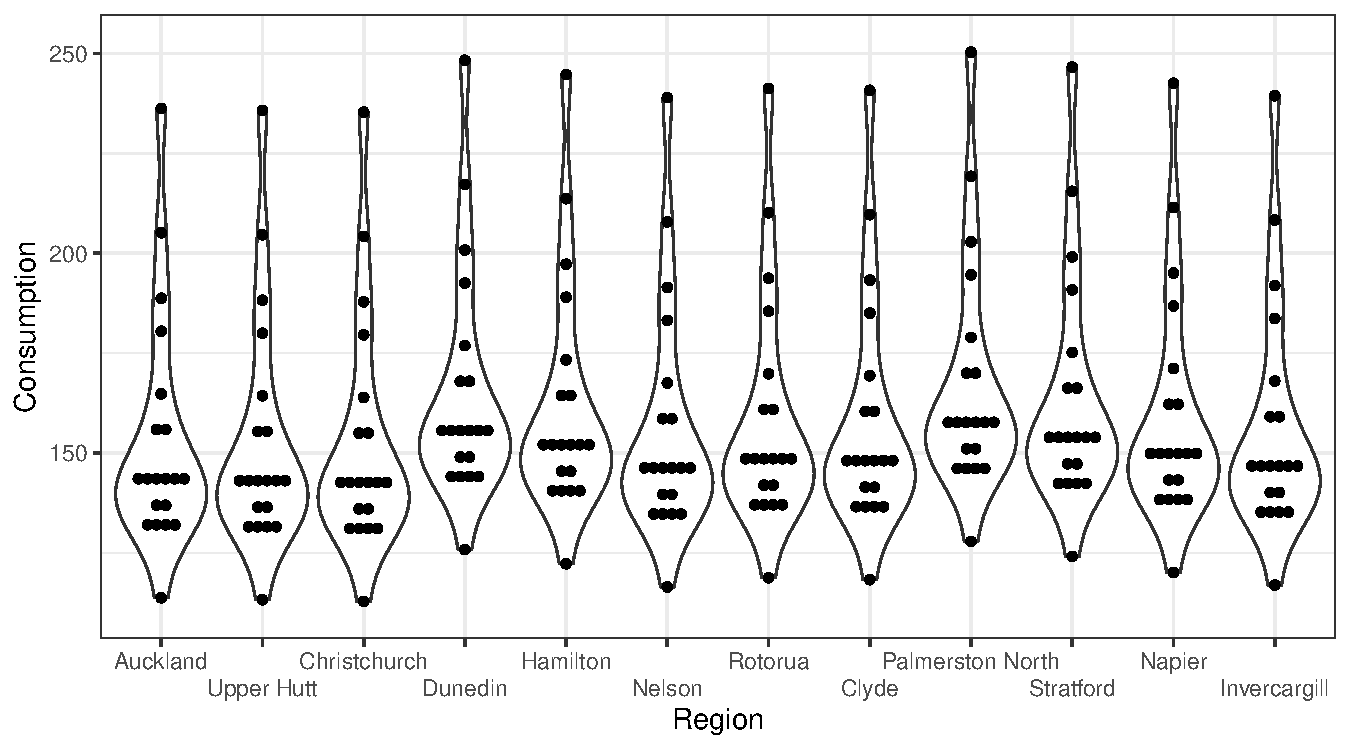
\includegraphics{final_report_Raffertys_edits_for_Vector_files/figure-latex/consum_den-1.pdf}
\caption{Distribution of linear model coeffients (``baseline'' energy
economy by model for each region)\label{fig:consum_den}}
\end{figure}

\hypertarget{predictions}{%
\subsection{Predictions}\label{predictions}}

We can use the above model to explore future electric vehicle charging
electricity demand. To do this we make the following assumptions:

\begin{itemize}
\item Going forward, regional VKT remains relatively consistent with 2019 VKT data. 
\item Regional weather data from 2017 to 2021 remains consistent with future climate of NZ.
\item Flip the Fleet's vehicle make-up is representative of NZs future EV fleet (although we explore some extreme cases).
\item Actual VKT of each region remains relatively constant throughout the year.
\end{itemize}

\begin{figure}
\centering
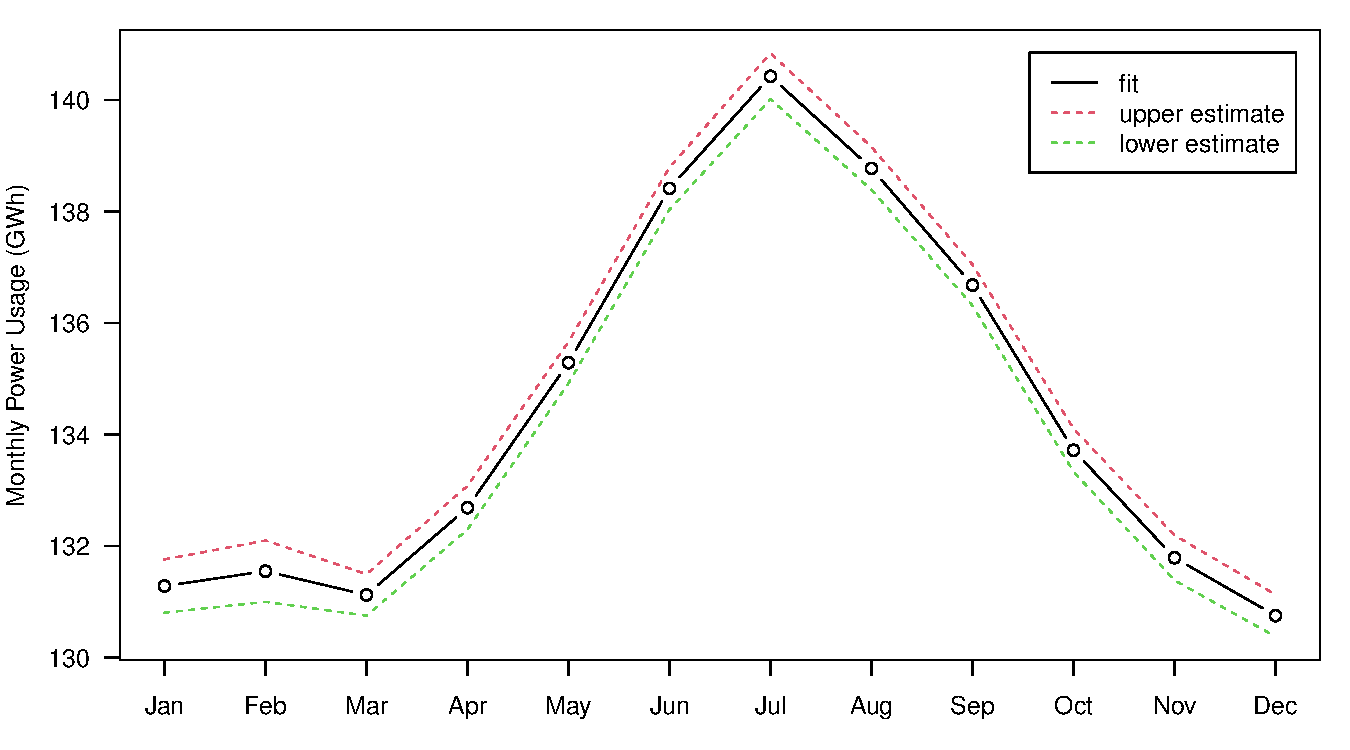
\includegraphics{final_report_Raffertys_edits_for_Vector_files/figure-latex/Auckland_power-1.pdf}
\caption{Auckland region 100\% EV case total EV electricity demand per
month\label{fig:Auckland_power}}
\end{figure}

Combining Auckland only Ministry of Transport 2019 VKT with the energy
economy linear model using Flip the Fleet's vehicle make up and average
weather data from 2017-2021 we can estimate the electricity demand for
Auckland under a 100\% EV uptake (Figure \ref{fig:Auckland_power}). The
estimated EV electricity demand per month shows a clear seasonal trend
from around 127.7 GWh per month in summer to around 137.1 GWh per month
in the winter.

\begin{figure}
\centering
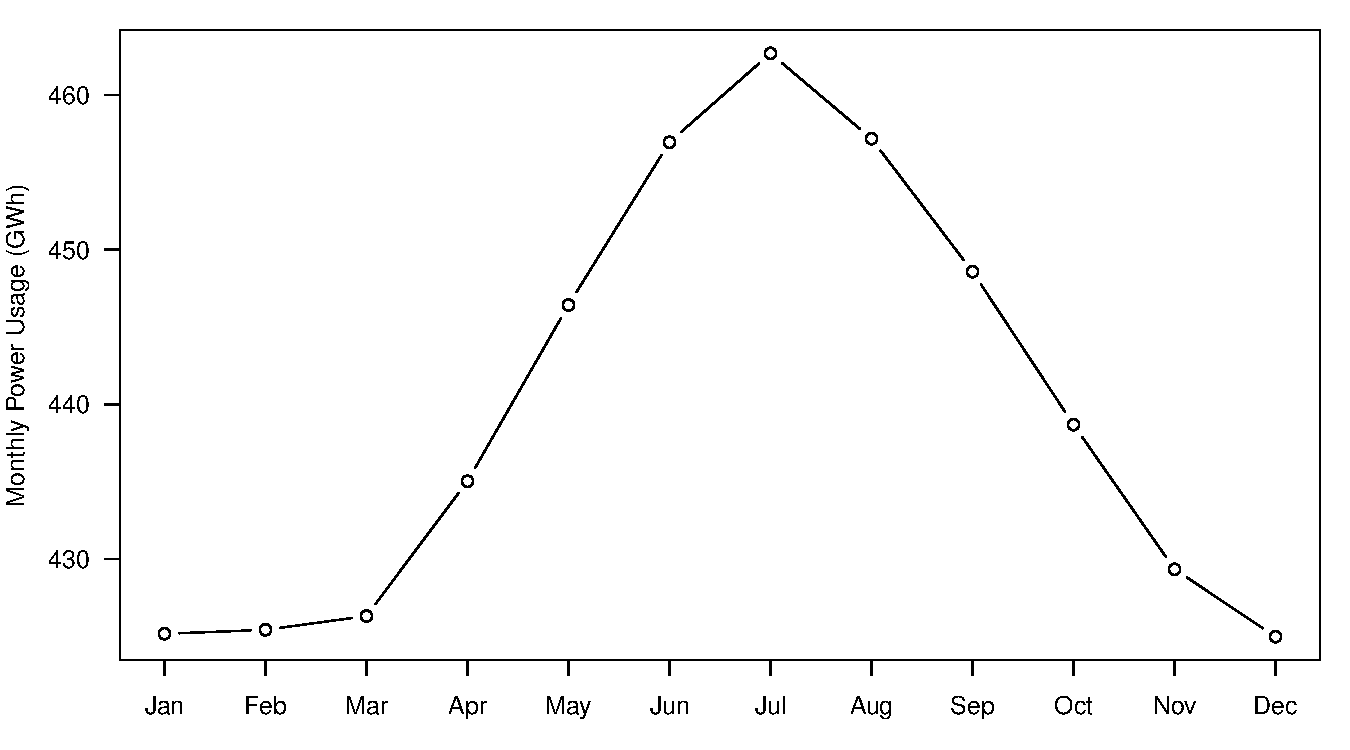
\includegraphics{final_report_Raffertys_edits_for_Vector_files/figure-latex/NZ_power-1.pdf}
\caption{NZ 100\% EV case total EV electricity demand per
month\label{fig:NZ_power}}
\end{figure}

Similarly, combining all Ministry of Transport 2019 VKT with the energy
economy linear model using Flip the Fleets vehicle make up and average
regional weather data from 2017-2021 we can determine the electricity
demand for all NZ with 100\% EV uptake (Figure \ref{fig:NZ_power}). A
clear seasonal trend can be observed from around 416 GWh per month in
summer to around 453 GWh per month in the winter.

\begin{figure}
\centering
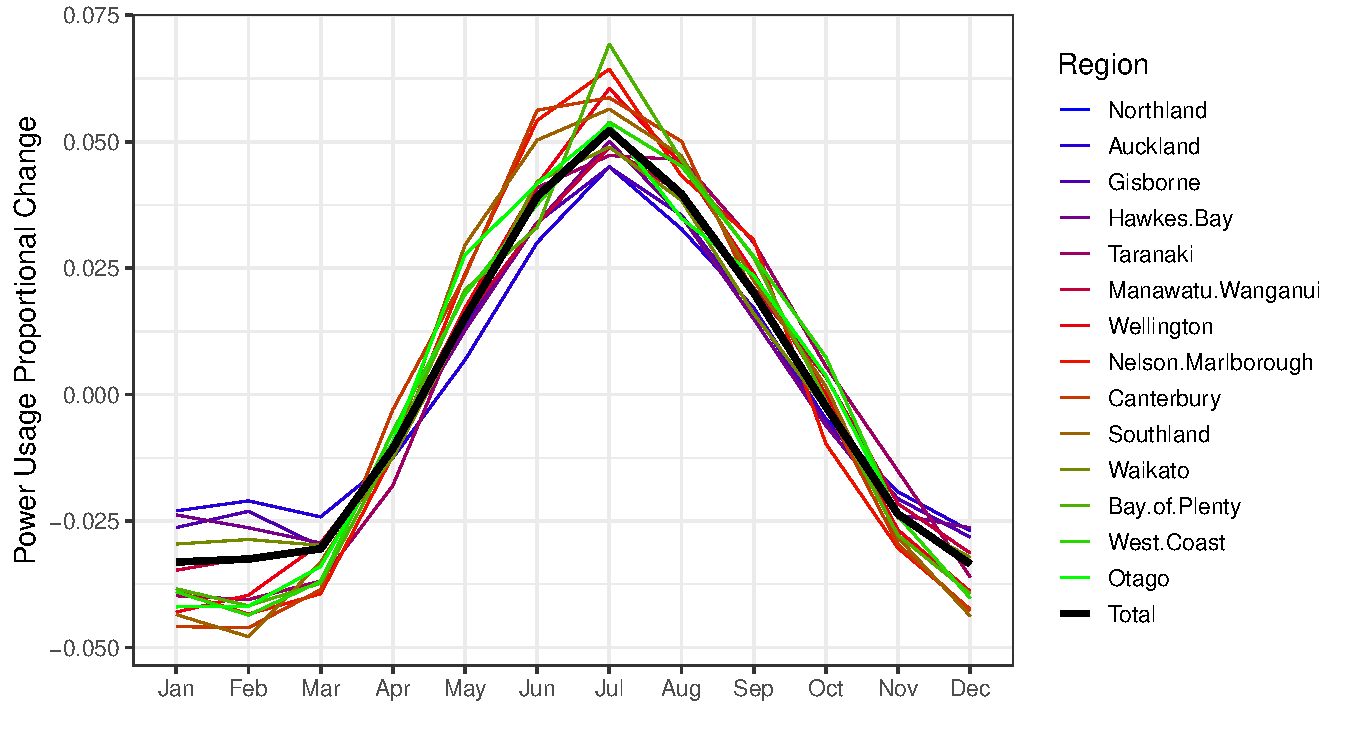
\includegraphics{final_report_Raffertys_edits_for_Vector_files/figure-latex/NZ_region_power_prop-1.pdf}
\caption{All NZ regions monthly proportional change in EV electricity
demand relative to its yearly average\label{fig:NZ_region_power_prop}}
\end{figure}

Applying the same process to all regions individually we can also plot
each regions proportional change in EV electricity demand relative to
its yearly average. Figure \ref{fig:NZ_region_power_prop} shows all
regions follow a similar seasonal change in power energy economy. Of
note, warmer regions like Northland and Auckland appear to have less of
a seasonal trend compared to regions such as Otago and the West Coast.

\begin{figure}
\centering
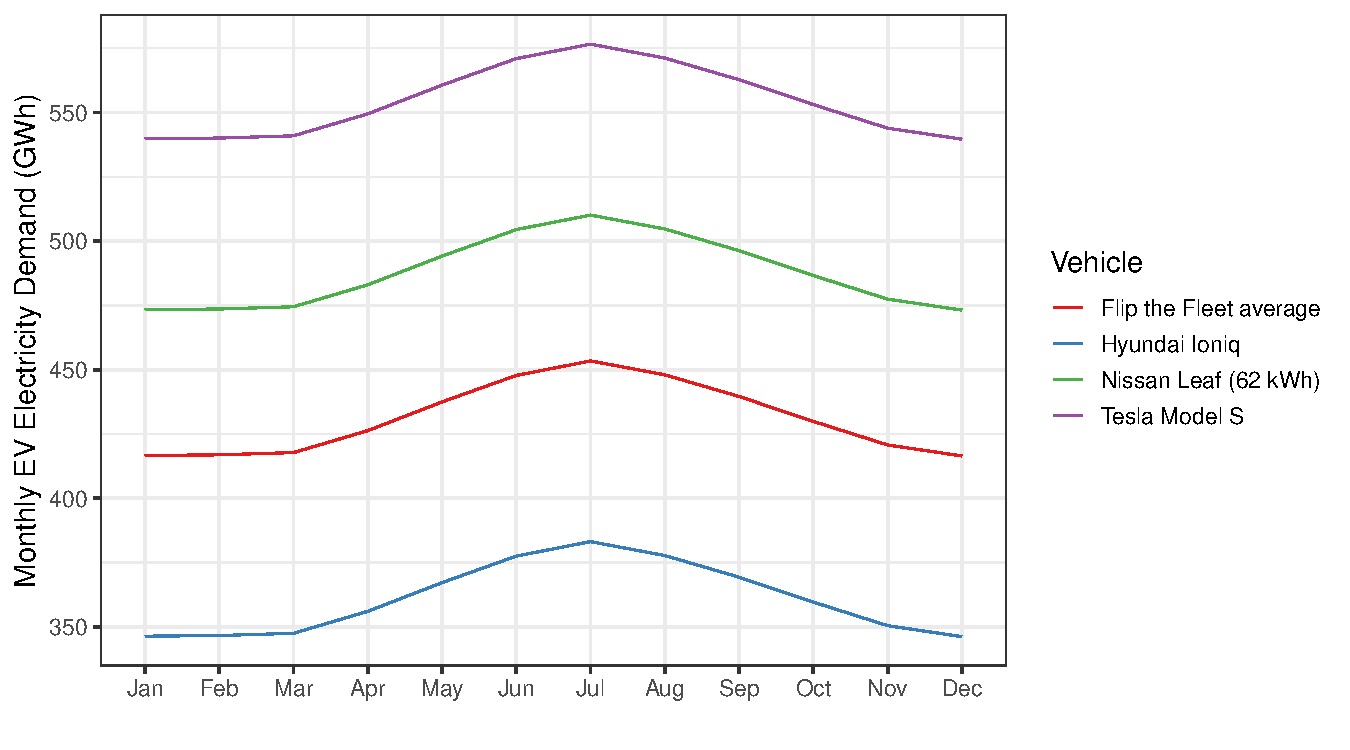
\includegraphics{final_report_Raffertys_edits_for_Vector_files/figure-latex/vehicle_power_usage-1.pdf}
\caption{2019 VKT 100\% EV case NZ total EV electricity demand scenarios
by vehicle fleet model makeup\label{fig:vehicle_power_usage}}
\end{figure}

Combining the regional energy economy with the 2019 VKT number we can
get an expected EV electricity demand for all of NZ and also for each
VKT region. Figure \ref{fig:vehicle_power_usage} shows with a 100\% EV
penetration and an EV fleet comparable to the Flip the Fleet, the
monthly EV electricity demand for all of NZ goes from 416 GWh in the
summer to 453 GWh in the winter. If the fleet consisted of heavier less
efficient vehicles like the Tesla Model S this would increase to 540 GWh
in the summer and 577 GWh in the winter.

\begin{figure}
\centering
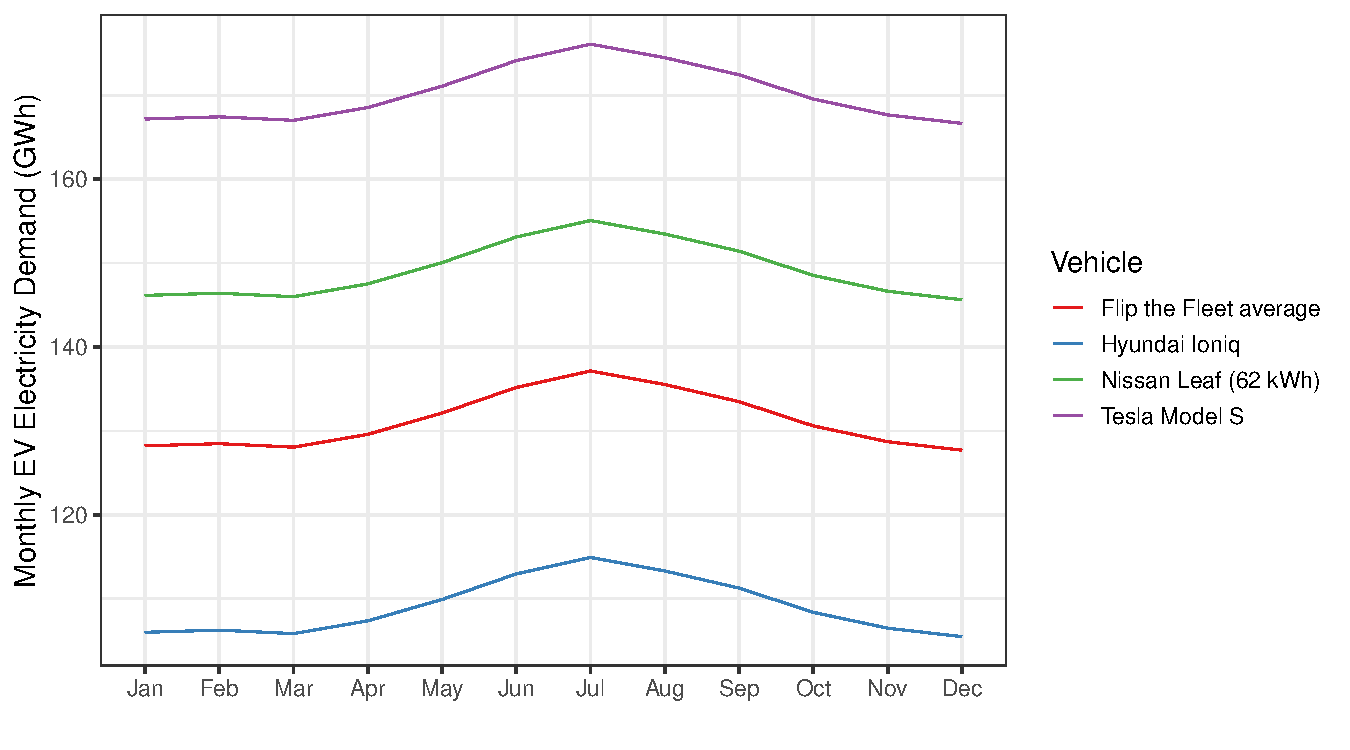
\includegraphics{final_report_Raffertys_edits_for_Vector_files/figure-latex/vehicle_power_usage_auck-1.pdf}
\caption{2019 VKT 100\% EV case Auckland total EV electricity demand
Scenarios by vehicle fleet model
makeup\label{fig:vehicle_power_usage_auck}}
\end{figure}

Figure \ref{fig:vehicle_power_usage_auck} shows with a 100\% EV
penetration and an EV fleet comparable to that of Flip the Fleet, the
monthly EV electricity demand of Auckland goes from 128 GWh in the
summer to 137 GWh in the winter. If the fleet consisted of heavier less
efficient vehicles like the Tesla Model S this would increase to 167 GWh
minimum in the summer and 176 GWh in the winter.

Figures \ref{fig:vehicle_power_usage} and
\ref{fig:vehicle_power_usage_auck} show that the vehicle make up of the
fleet may have a much greater impact than other variables on the total
energy demand that EVs will have on the network.

\hypertarget{comparison-and-incorporation-of-times-model-predictions}{%
\subsubsection{Comparison and Incorporation of Times Model
Predictions}\label{comparison-and-incorporation-of-times-model-predictions}}

To compare our predictions and see how they fit in with other well
established models, ECCA Times Model \cite{times_model} is used as a
comparison. For this, VKT and expected power usage by passenger vehicle
EVs for selected years between 2018 to 2060 was downloaded from EECA.
Expected energy economy (Wh/km) assumed by ECCA was then calculated by
dividing power usage by VKT.

\begin{figure}
\centering
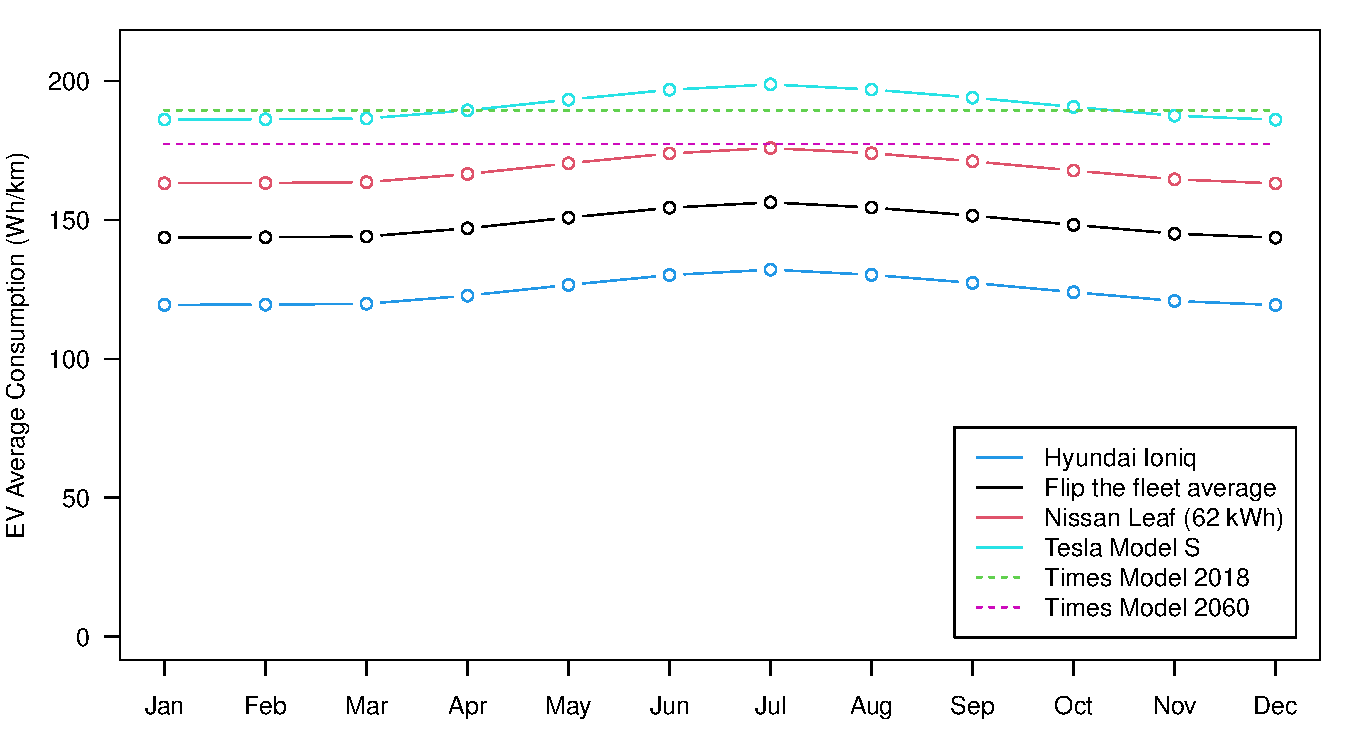
\includegraphics{final_report_Raffertys_edits_for_Vector_files/figure-latex/vehicle_consum-1.pdf}
\caption{NZ vehicle average energy economy
scenarios\label{fig:vehicle_consum}}
\end{figure}

Figure \ref{fig:vehicle_consum} compares Flip the Fleet energy economy
values to the energy economy assumed in EECA's times Tui model
\cite{times_model}. We can see that ECCA's times model assumes a much
higher energy economy (lower efficiency) than the Flip the Fleet data
suggests is common in NZ. Modelling the Flip the Fleet vehicle make up
suggests an average energy economy of 148.6Wh/km. However, this is
consisting primarily of Nissan leafs (1078 out of 1264 vehicles), which
are a comparatively light and efficient EV. The 2018 times model energy
economy is much more comparable to much heavier and less efficient Tesla
Model S (based on 81 months of efficiency data from 5 vehicles).

\begin{figure}
\centering
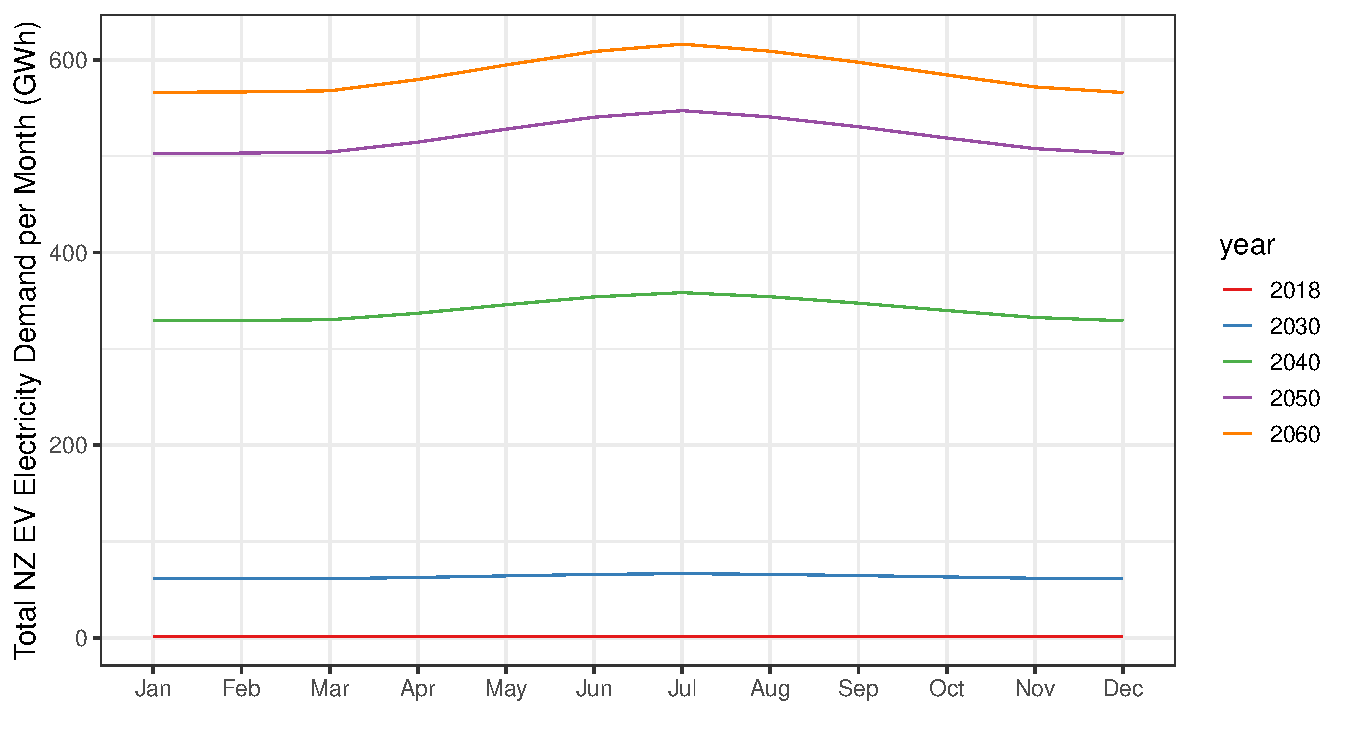
\includegraphics{final_report_Raffertys_edits_for_Vector_files/figure-latex/kea_power_usage-1.pdf}
\caption{NZ EVs electricity demand per month using EECAs Kea VKT and
Flip the Fleets average energy economy\label{fig:kea_power_usage}}
\end{figure}

\begin{figure}
\centering
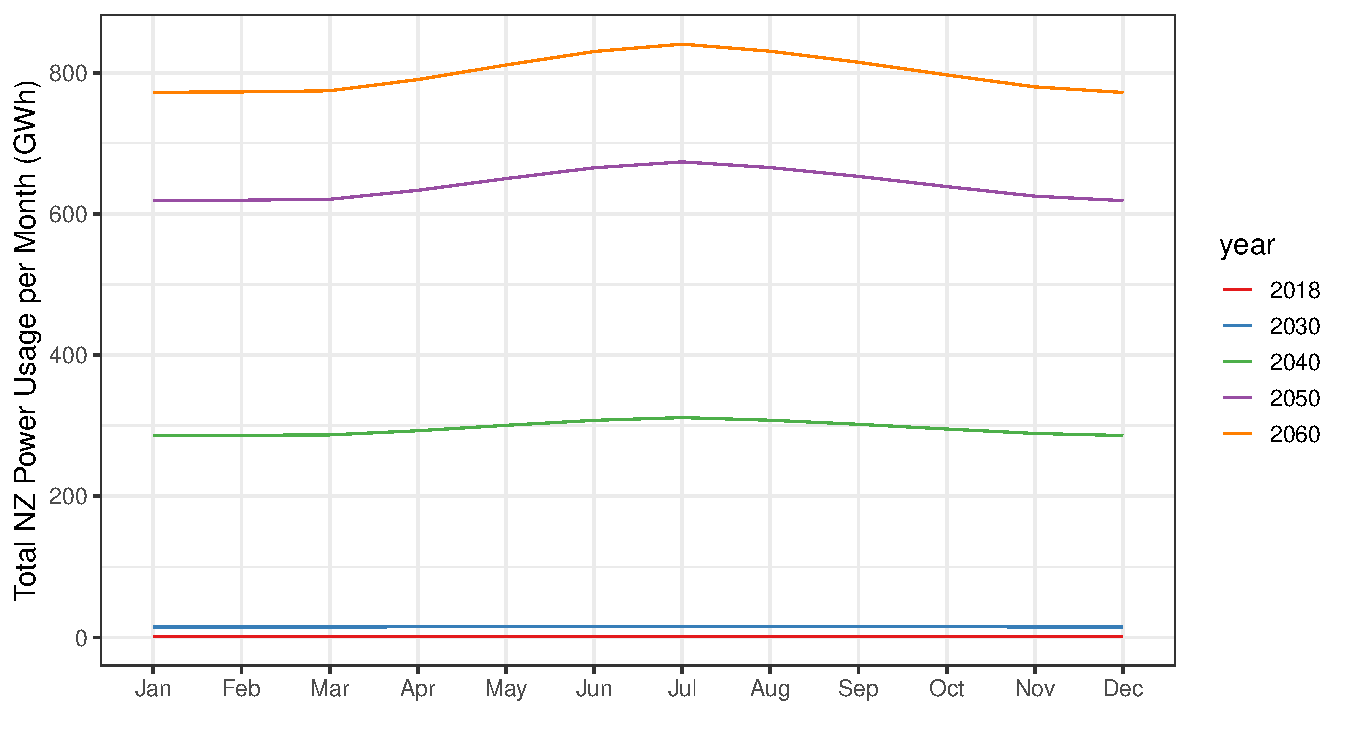
\includegraphics{final_report_Raffertys_edits_for_Vector_files/figure-latex/tui_power_usage-1.pdf}
\caption{NZ EVs electricity demand per month using EECAs Tui VKT and
Flip the Fleets average energy economy\label{fig:tui_power_usage}}
\end{figure}

Figures \ref{fig:kea_power_usage} and \ref{fig:tui_power_usage} use our
energy economy model with Flip the Fleets vehicle make up, NZ region
weather from 2017 to 2021 and Ministry of Transport VKT regional
proportions combined with ECCA times models expected passenger EV VKT to
estimate total monthly power usage of NZ by passenger EVs for select
years between 2018 and 2060. These show that under current or
near-future EV uptakes, seasonal variation in EV demand will be
negligible when considering their percentage of total electricity
consumption. However, beyond 2040 the seasonal variation in EV demand
will be more substantial, and should be considered when designing the
electricity netowrk of the future.

\begin{thebibliography}{9}
\bibitem{ftf}
\textit{Flip the Fleet Website}
\\\texttt{https://flipthefleet.org/}
\bibitem{ev_range}
\textit{To what degree does temperature impact EV range?}
\\\texttt{\url{https://www.geotab.com/blog/ev-range/}}
\bibitem{ev_highway}
\textit{Why is the range of an EV less on the freeway than the city?}
\\\texttt{\url{https://evcentral.com.au/why-is-the-range-of-an-ev-less-on-the-freeway-than-the-city/}}
\bibitem{fuel_trade}
\textit{MBIE oil trade statistics}
\\\texttt{\url{https://www.mbie.govt.nz/building-and-energy/energy-and-natural-resources/energy-statistics-and-modelling/energy-statistics/oil-statistics/}}
\bibitem{HDD_est}
\textit{Bayesian estimation of a building's base temperature for the calculation of heating degree-days}
\\\texttt{\url{https://www.sciencedirect.com/science/article/abs/pii/S0378778816312907}}
\bibitem{NZTA_VKT}
\textit{Ministry of Transport VKT data website}
\\\texttt{\url{https://www.transport.govt.nz/statistics-and-insights/fleet-statistics/vehicle-kms-travelled-vkt-2/}}
\bibitem{times_model}
\textit{ECCA Times Model}
\\\texttt{\url{https://www.eeca.govt.nz/insights/data-tools/new-zealand-energy-scenarios-times-nz/}}
\end{thebibliography}

\end{document}
